%%%%%%%%%%%%%%%%%%%%%%%%%%%%%%%%%%%%%%%%%%%%%%%%%%%%%%%%%%%%%%%%%%%%
%% I, the copyright holder of this work, release this work into the
%% public domain. This applies worldwide. In some countries this may
%% not be legally possible; if so: I grant anyone the right to use
%% this work for any purpose, without any conditions, unless such
%% conditions are required by law.
%%%%%%%%%%%%%%%%%%%%%%%%%%%%%%%%%%%%%%%%%%%%%%%%%%%%%%%%%%%%%%%%%%%%

\documentclass[
  digital, %% This option enables the default options for the
           %% digital version of a document. Replace with `printed`
           %% to enable the default options for the printed version
           %% of a document.
  oneside, %% This option enables double-sided typesetting. Use at
           %% least 120 g/m² paper to prevent show-through. Replace
           %% with `oneside` to use one-sided typesetting; use only
           %% if you don’t have access to a double-sided printer,
           %% or if one-sided typesetting is a formal requirement
           %% at your faculty.
  table,   %% This option causes the coloring of tables. Replace
           %% with `notable` to restore plain LaTeX tables.
  lof,     %% This option prints the List of Figures. Replace with
           %% `nolof` to hide the List of Figures.
  nolot,     %% This option prints the List of Tables. Replace with
           %% `nolot` to hide the List of Tables.
  %% More options are listed in the user guide at
  %% <http://mirrors.ctan.org/macros/latex/contrib/fithesis/guide/mu/fi.pdf>.
]{fithesis3}
\usepackage{gensymb}
\usepackage{subcaption}
%% The following section sets up the locales used in the thesis.
\usepackage[resetfonts]{cmap} %% We need to load the T2A font encoding
\usepackage[T1,T2A]{fontenc}  %% to use the Cyrillic fonts with Russian texts.
\usepackage[
  main=slovak, %% By using `czech` or `slovak` as the main locale
                %% instead of `english`, you can typeset the thesis
                %% in either Czech or Slovak, respectively.
  english, german, russian, czech, slovak %% The additional keys allow
]{babel}        %% foreign texts to be typeset as follows:
%%
%%   \begin{otherlanguage}{german}  ... \end{otherlanguage}
%%   \begin{otherlanguage}{russian} ... \end{otherlanguage}
%%   \begin{otherlanguage}{czech}   ... \end{otherlanguage}
%%   \begin{otherlanguage}{slovak}  ... \end{otherlanguage}
%%
%% For non-Latin scripts, it may be necessary to load additional
%% fonts:
\usepackage{paratype}
\def\textrussian#1{{\usefont{T2A}{PTSerif-TLF}{m}{rm}#1}}
%%
%% The following section sets up the metadata of the thesis.
\thesissetup{
    date          = \the\year/\the\month/\the\day,
    university    = mu,
    faculty       = fi,
    type          = bc,
    author        = Henrieta Micheľová,
    gender        = f,
    advisor       = {prof. RNDr. Ivana Černá, CSc.},
    title         = {Distribuované algoritmy pro rekonfiguraci platformy RoFI},
    TeXtitle      = {Distribuované algoritmy pro rekonfiguraci platformy RoFI},
    keywords      = {modulárny, robot, distribuovaný, algoritmus, rekonfigurácia, platforma RoFI, MPI, openMPI},
    TeXkeywords   = {modulárny, robot, distribuovaný, algoritmus, rekonfigurácia, platforma RoFI, MPI, openMPI},
    abstract      = {Platforma RoFI je nová modulárna robotická platforma vyvíjaná v laboratóriu ParaDiSe. Táto práca stavia na už definovaných konceptoch platformy a prináša nový pohľad na rekonfigurácie modularnych robotov tejto platformy. Táto práca navrhuje a implementuje riešenie problému rekonfigurácie robotov z distribuovaného hľadiska, teda z pohľadu jedného modulu platformy na problém rekonfigurácie celého robota. Táto práca prezentuje nástroj \textit{rofi-distribute}, ktorý poskytuje dva algoritmy na simuláciu distribuovanej rekonfigurácie, ktoré boli ostatestované na množstve príkladov. Výsledkami práce sú porovnanie navrhnutých algoritmov medzi sebou navzájom, ale aj porovnanie voči centralizovanému riešeniu problému rekonfigurácia z pohľadu času výpočtov a dĺžok samotných rekonfigurácií. },
    thanks        = {Veľká vďaka patrí všetkým ľudom v laboratóriu ParaDiSe za príjemnú atmosféru pri práci a každodennú čokoládu, hlavne celému tímu, ktorý sa podieľa na vývoji platformy RoFI, a to hlavne vedúcej práce Ivane Černej a ďalším členom: Jiřímu Barnatovi, Janovi Mrázkovi, Viktórii Vozárovej a Markéte Naušovej, ktorí boli vždy ochotní zodpovedať mi otázky, prípadne konzultovať nápady. 
    
    Rovnaká vďaka patrí aj Vladimírovi Štillovi za pohotovú pomoc pri technických komplikáciách a Lukášovi Korenčikovi za podporu pri práci počas sviatkov a víkendov. V neposlednom rade aj Tomášovi Szaniszlovi za podporu a korekcie textu práce do neskorých nočných hodín. A aj rodine a kamarátom za ich podporu nielen pri tvorbe tejto práce. },
    bib           = bibliography.bib,
}
\usepackage{makeidx}      %% The `makeidx` package contains
\makeindex                %% helper commands for index typesetting.
%% These additional packages are used within the document:
\usepackage{paralist} %% Compact list environments
\usepackage{amsmath}  %% Mathematics
\usepackage{amsthm}
\usepackage{amsfonts}
\usepackage{url}      %% Hyperlinks
\usepackage{markdown} %% Lightweight markup
\usepackage{listings} %% Source code highlighting
\lstset{
  basicstyle      = \ttfamily,%
  identifierstyle = \color{black},%
  keywordstyle    = \color{blue},%
  keywordstyle    = {[2]\color{cyan}},%
  keywordstyle    = {[3]\color{olive}},%
  stringstyle     = \color{teal},%
  commentstyle    = \itshape\color{magenta}}
\usepackage{floatrow} %% Putting captions above tables
\floatsetup[table]{capposition=top}

\usepackage{enumitem}
\setitemize{itemsep=-5pt,topsep=10pt,parsep=10pt,partopsep=10pt}
\setenumerate{itemsep=-5pt,topsep=10pt,parsep=10pt,partopsep=10pt}
\usepackage[slovak,linesnumbered,ruled,vlined]{algorithm2e}
\newtheorem{lemma}{Lemma}
\usepackage{minted}

\usepackage{color}
\definecolor{modra}{rgb}{0,0,1}
\definecolor{zlta}{rgb}{1,1,0}
\definecolor{cervena}{rgb}{1,.2706,.2667}
    
\begin{document}
\chapter*{Úvod}
\addcontentsline{toc}{chapter}{Úvod}
-- napisat strukturu celej prace!

% ------------------------------------------------------ 1 ------------------------------------------------------
\chapter{Popis platformy RoFI}
\label{sec:platform}
RoFI je modulárna robotická platforma, ktorá vzniká na pôde Fakulty informatiky Masarykovej univerzity v laboratóriu ParaDiSe\footnote{skratka pre Laboratoř paralelních a distribuovaných systémů (stránka laboratória: \url{https://paradise.fi.muni.cz/})}. Táto platforma zastrešuje vývoj modulárnych robotov a iného príslušenstva po ich hardvérovej, ale aj softvérovej stránke na rôznych úrovniach. 

Primárnym cieľom platformy RoFI je vytvorenie modulárnych robotov, ktoré je možné využiť na rôzne úlohy. Príkladom sú úlohy ako prechádzanie cez úzke priestory, prekonávanie prekážok a podobne. 

Ich dizajn je navrhovaný tak, aby bolo jednoduché a nie príliš finančne náročné ich fyzicky skonštruovať. Softvérové vybavenie pokrýva široké spektrum požiadaviek modulárnych robotov a má jednoduché použitie pre užívateľov na rôznych úrovniach. 

Platforma je navrhnutá tak, aby bola ľahko rozšíriteľná o dodatočné periférie a pasívne prvky. Celý vývoj prebieha ako open-source projekt \cite{rofiGit}. 

Základnou jednotkou platformy RoFI sú moduly \cite{mrazekMasterThesis}, ktoré sú schopné sa vzájomne fyzicky prepojiť a zároveň medzi sebou komunikovať \cite{rofiCom}. Okrem toho sa každý modul dokáže pripojiť aj na pasívne prvky. 

Prepojenie viacerých modulov umožňuje vytvoriť tzv. RoFIbotov \cite{rofiWeb}, ktoré majú širšie spektrum funkcionalít ako samostatné moduly. Cieľom tejto práce je práve zamerať sa na RoFIbotov a ich schopnosť rekonfigurovať sa za špecifických podmienok. 

Pre účel tejto práce je popísaná iba časť hardvérového vybavenia modulu a schopnosti prepájania modulov. Ďalšie rozšírenia, softvérové vybavenie a iné komponenty a návody sa nachádzajú na stránkach platformy \cite{rofiWeb}.

\section{Popis modulu}
\label{sec:moduleSpec}
RoFIbota je možné umiestniť do 3D siete tak, že každý modul sa nachádza v práve dvoch políčkach siete (tzv. \textit{lattice type}). Toto rozdelenie je navrhnuté tak, že každá z jeho dvoch strán (side) sa nachádza v práve jednom políčku (popis tvaru modulu sa nachádza nižšie). 

Toto umiestnenie do 3D mriežky spôsobuje, že tvar modulu je prispôsobený tak, aby pri pohybe zasahoval do najnižšieho možného počtu políčok siete (tzv. \textit{grid-awareness} \cite{mrazekMasterThesis}). 

V súčasnej dobe je platforma RoFI prispôsobená na mriežku s veľkosťou $10$\,cm. Podrobný popis vlastností modulu sa nachádza v diplomovej práci \textit{RoFI – Distributed Metamorphic Robots} \cite{mrazekMasterThesis}. 

\begin{figure}[hbt!]
    \centering
    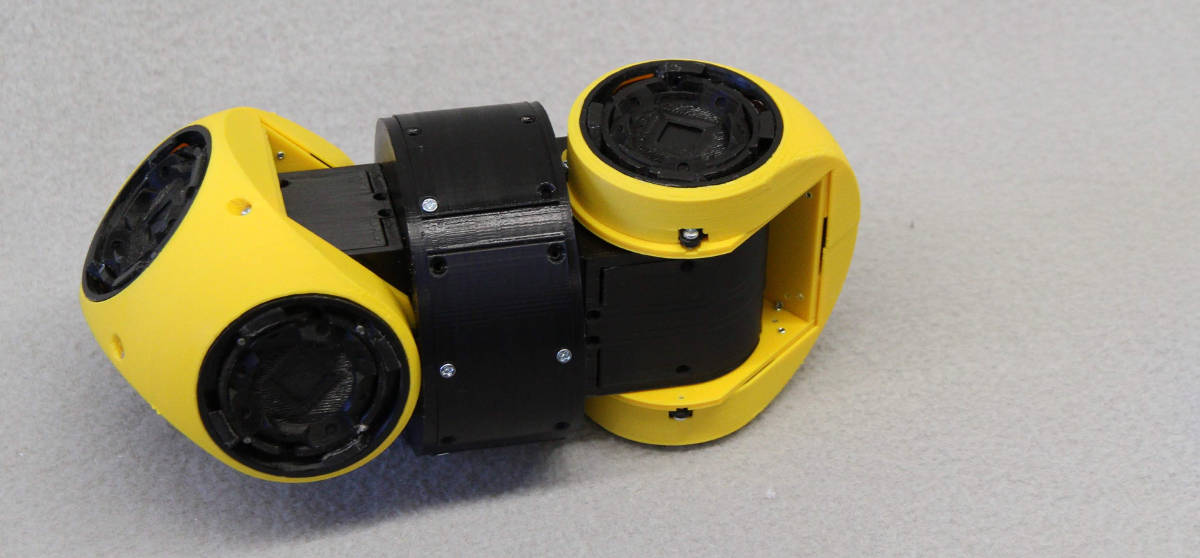
\includegraphics[width=0.6\textwidth]{pictures/module.jpg}
    \caption[Fotografia modulu]{Fotografia modulu \cite{rofiWeb}.}
    \label{fig:module}
\end{figure}

Každý z modulov sa skladá zo \textit{strany A} (\textit{side A}) a \textit{strany B} (\textit{side B}). Každá z nich sa delí na dve časti označené ako \textit{telo} (\textit{body}) a \textit{topánka} (\textit{shoe}) (viď obrázok \ref{fig:module_parts}). 

\begin{figure}[hbt!]
    \centering
    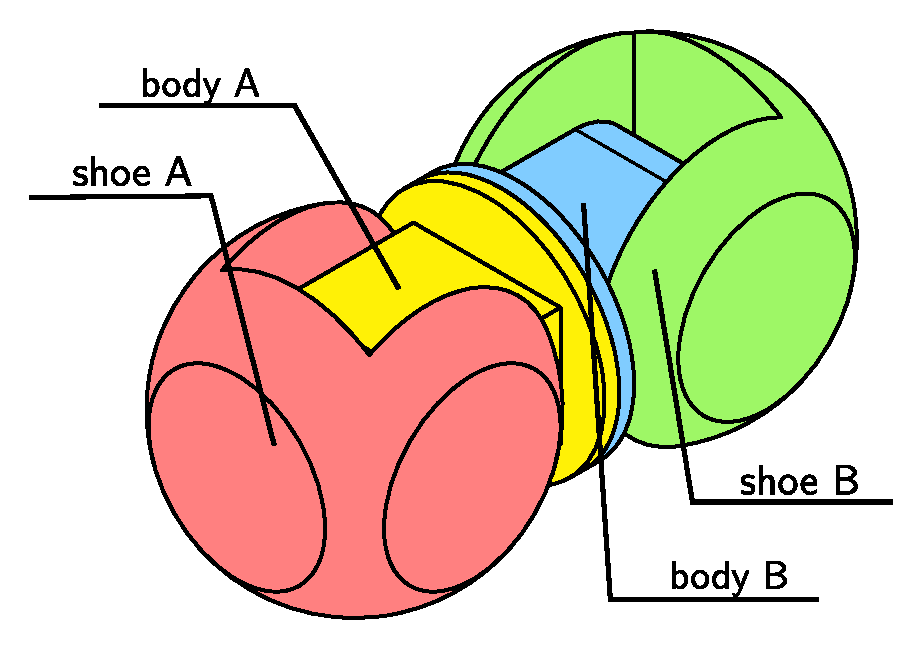
\includegraphics[width=0.6\textwidth]{pictures/module_parts.pdf}
    \caption[Časti modulu]{Schéma častí modulu \cite{mrazekMasterThesis}.}
    \label{fig:module_parts}
\end{figure}

Moduly majú schopnosť pohybovať sa, a to vďaka až trom stupňom voľnosti. Prvé dva z nich umožňujú pohybovať s časťou modulu označenou ako topánka. Konkrétne ide o pohyb okolo osí označovaných ako $\alpha$ a $\beta$ o uhol v rozsahu $\interval[{-90\degree, 90\degree}]$. Posledným stupňom voľnosti je pohyb okolo osi označovanej ako $\gamma$. Tento pohyb umožňuje otáčaním meniť vzájomnú polohu častí tiel modulu a jeho rozsah je $\interval({-180\degree, 180\degree}]$. 

\begin{figure}[hbt!]
    \centering
    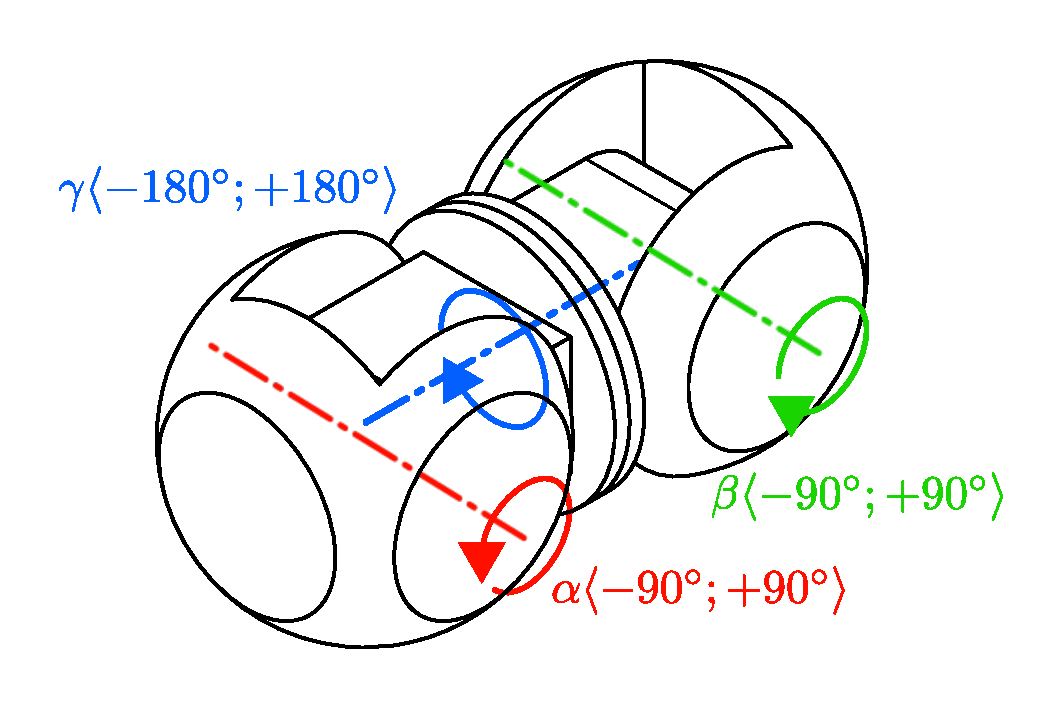
\includegraphics[width=0.6\textwidth]{pictures/module_angles.pdf}
    \caption[Stupne voľnosti modulu]{Schéma stupňov voľnosti modulu a smerov otáčania \cite{mrazekMasterThesis}.}
    \label{fig:module_angle}
\end{figure}

Ako bolo spomenuté vyššie, tak každý modul má schopnosť pripojiť sa k iným modulom (a vytvoriť tak RoFIbotov) alebo k pasívnym prvkom pomocou \textit{konektor}ov (\textit{dock}). Konektorový systém platformy RoFI je navrhnutý ako tzv. \textit{genderless}, čo umožňuje vzájomné spojenie ľubovoľných dvoch konektorov. 

Každý modul obsahuje práve šesť konektorov, ktoré sú rozmiestnené po tri na každej topánke modulu. Konektor je okrem svojej polohy na module definovaný aj orientačným vektorom (viď obrázok \ref{fig:dock_desc}). 

\begin{figure}[hbt!]
    \centering
    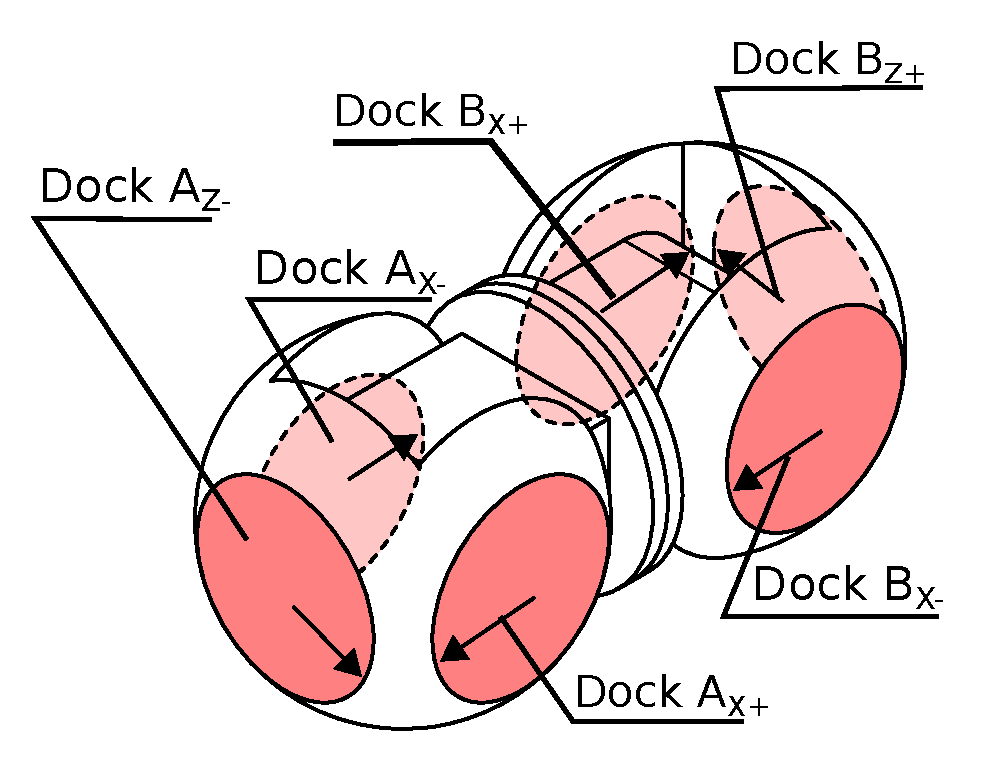
\includegraphics[width=0.6\textwidth]{pictures/dock_desc.pdf}
    \caption[Docky modulu]{Schéma umiestnení konektorov na module a ich označenia. Šípky na konektoroch znázorňujú orientačné vektory \cite{mrazekMasterThesis}.}
    \label{fig:dock_desc}
\end{figure}

Prepojenie je definované vzájomnou polohou orientačných vektorov konektorov spojenia. Konštrukcia konektorov dovoľuje ich prepojenie až v štyroch rôznych polohách. 

Vzájomná poloha orientačných vektorov konektorov môže byť postupne $0\degree$, $90\degree$, $180\degree$ alebo $270\degree$ a tieto prepojenia sa označujú v tomto poradí ako \textit{North}, \textit{East}, \textit{South} a \textit{West} (viď obrázok \ref{fig:dock_orientation}). 

\begin{figure}[hbt!]
    \centering
    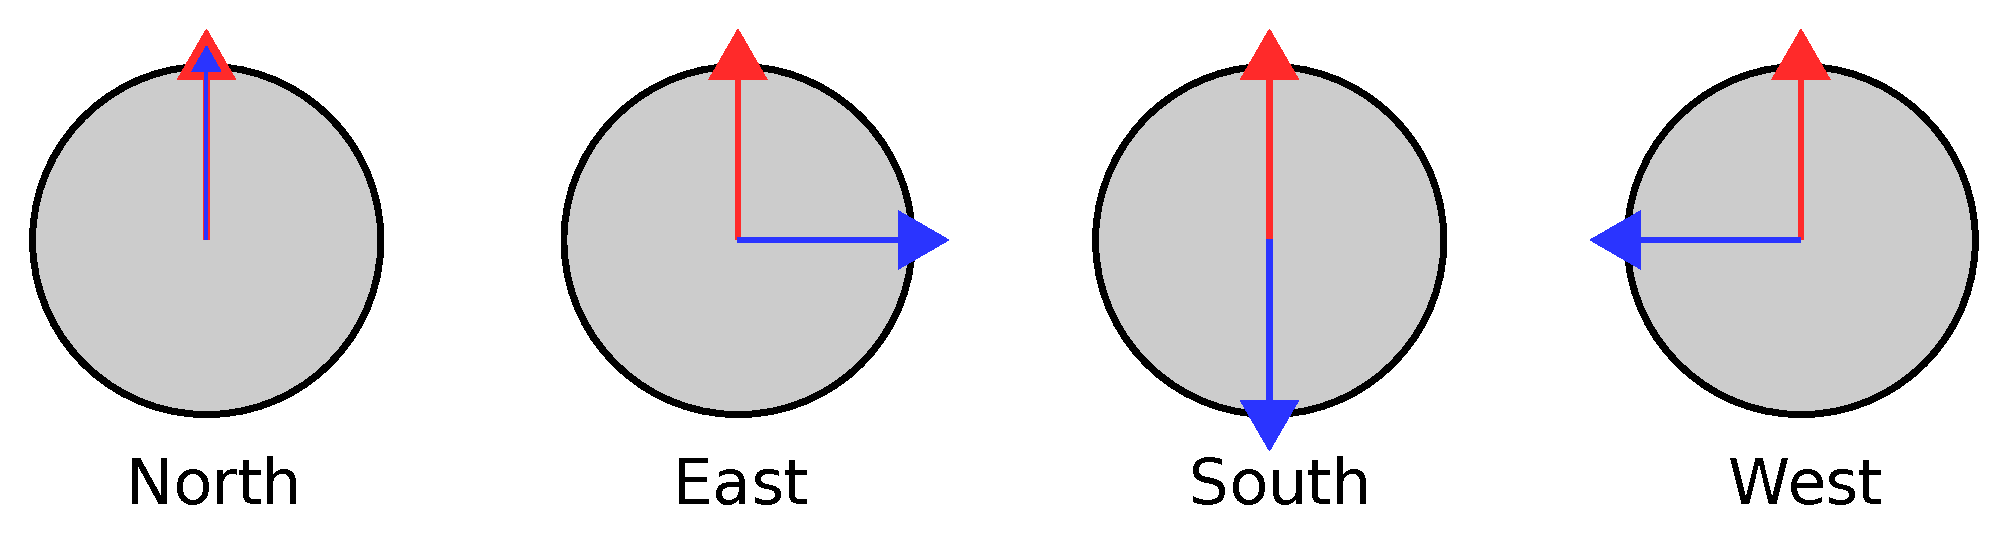
\includegraphics[width=0.6\textwidth]{pictures/dock_orientation.pdf}
    \caption[Poloha prepojenia konektorov modulu]{Schéma vzájomnej polohy orientačných vektorov spojených konektorov modulov. Červenou je označený konektor modulu, z ktorého perspektívy spojenie označujeme. Modrá šípka je orientačný vektor druhého modulu. Poznámka: nezáleží na výbere konektoru, z ktorého perspektívy spojenie sledujeme \cite{mrazekMasterThesis}.}
    \label{fig:dock_orientation}
\end{figure}

\section{Popis RoFIbota}
\label{sec:rofibotSpec}
Vzájomné prepojenie modulov pomocou konektorov vytvára RoFIbotov. Parametre RoFIbota, ktoré ho definujú, sa dajú rozdeliť do dvoch kategórií:   
\begin{enumerate}
    \item tvar RoFIbota vzhľadom na jeho vnútornú štruktúru:
    \begin{itemize}[topsep=-5pt]
        \item množina modulov RoFIbota, 
        \item množina prepojení (hrán) modulov; 
    \end{itemize}
    
    \item poloha RoFIbota vzhľadom k okolitému svetu: 
    \begin{itemize}[topsep=-5pt]
        \item natočenie celého RoFIbota vzhľadom na okolie, 
        \item umiestnenie RoFIbota do priestoru.  
    \end{itemize}
\end{enumerate}

\textit{Konfigurácia} RoFIbota je tvar RoFIbota vzhľadom na jeho vnútornú štruktúru, teda množina modulov a ich prepojení. Každý modul v konfigurácii RoFIbota je definovaný jedinečným identifikátorom modulu a hodnotami všetkých troch stupňov voľnosti modulu. 

Jednotlivé hrany (prepojenia) v konfigurácii RoFIbota sú definované identifikátormi spojených modulov a presným popisom konektorov, ktorými sú prepojené, a vzájomnou polohou spojených konektorov. 

\textit{Rekonfigurácia} RoFIbota je postupnosť validných krokov, ktorá u\-mož\-ní zmeniť počiatočnú konfiguráciu RoFIbota na cieľovú konfiguráciu RoFIbota. 
% ------------------------------------------------------ 1 ------------------------------------------------------






% ------------------------------------------------------ 2 ------------------------------------------------------
\chapter{Distribuovaná rekonfigurácia RoFIbotov}
\section{Formálna špecifikácia komponent}
\label{sec:formalSpec}
Fyzický stav modulu a konfigurácie RoFIbota je nutné popísať z formálneho hľadiska. Na základe tohto popisu je následne definovaná aj rekonfigurácia RoFIbota. 

\subsection{Modul}
\label{sec:formalSpecModul}
V prvom rade je nutné definovať \textit{stav modulu}, ktorý je tvorený nasledujúcimi údajmi: 
\begin{itemize}
    \item \textit{id} -- unikátny identifikátor modulu, 
    \item $\alpha$ -- uhol otočenia topánky A voči telu A v rozsahu $\interval[{-90\degree, 90\degree}]$,
    \item $\beta$ -- uhol otočenia topánky B voči telu B v rozsahu $\interval[{-90\degree, 90\degree}]$,
    \item $\gamma$ -- uhol otočenia tela A voči telu B v rozsahu $\interval({-180\degree, 180\degree}]$,
    \item sedmica o každom prepojení, ktoré daný modul má. 
\end{itemize} 

Ako už bolo popísané, tak spojenie definujú konektory, ktorými sú moduly spojené, a ich vzájomná poloha. Formálne ide o nasledujúcu sedmicu: 
\begin{itemize}
    \item \textit{id1} -- unikátny identifikátor prvého modulu, 
    \item \textit{side1} -- strana prvého modulu, ktorou je spojený s druhým modulom, 
    \item \textit{dock1} -- konektor prvého modulu, ktorý sa podieľa na prepojení,
    \item \textit{ori} -- orientácia spojených konektorov,
    \item \textit{dock2} -- konektor druhého modulu, ktorý sa podieľa na prepojení,
    \item \textit{side2} -- strana druhého modulu, ktorou je spojený s prvým modulom, 
    \item \textit{id2} -- unikátny identifikátor druhého modulu. 
\end{itemize}
Zároveň platí, že tieto hodnoty sú z množín: $side1, side2 \in \{A, B\}$; $dock1, dock2 \in \{+X, -X, -Z\}$; $ori \in \{N, E, S, W\}$.

\subsection{Konfigurácia}
\label{sec:formalSpecCfg}
Moduly sa spájajú do RoFIbotov a je nutné definovať si validitu konfigurácie. Konfigurácia RoFIbota je \textit{validná}, ak: 
\begin{itemize}
    \item každé prepojenie je vzájomné,
    \item každý konektor každého modulu sa podieľa na maximálne jednom prepojení, 
    \item všetky definované prepojenia je možné fyzicky vytvoriť (ich vzdialenosť dostatočne malá \cite{rofiCom}), 
    \item nesmie dochádzať k žiadnej fyzickej kolízii modulov. 
\end{itemize}
Formálny popis výpočtu kolízií v konfigurácii RoFIbota je podrobnejšie popísaný v diplomovej práci \textit{Motion Planning for the RoFI Platform} \cite{vozarovaMasterThesis}. 

Keďže komunikácia medzi modulmi môže prebiehať po fyzickom spojení pomocou konektorov, ale aj bezdrôtovo, tak si zadefinujeme spojitosť RoFIbota. 

RoFIbot je \textit{spojitý}, ak medzi akýmikoľvek jeho dvomi modulmi existuje cesta tvorená modulmi a prepojeniami. To značí, že komunikácia medzi akýmikoľvek dvomi modulmi spojitého RoFIbota môže prebiehať výhradne fyzickými spojeniami (viď príklad spojitej a nespojitej konfigurácie na obrázku \ref{fig:exampleCfg}). 

\begin{figure}[hbt!]
    \centering
    \begin{subfigure}[b]{0.49\textwidth}
        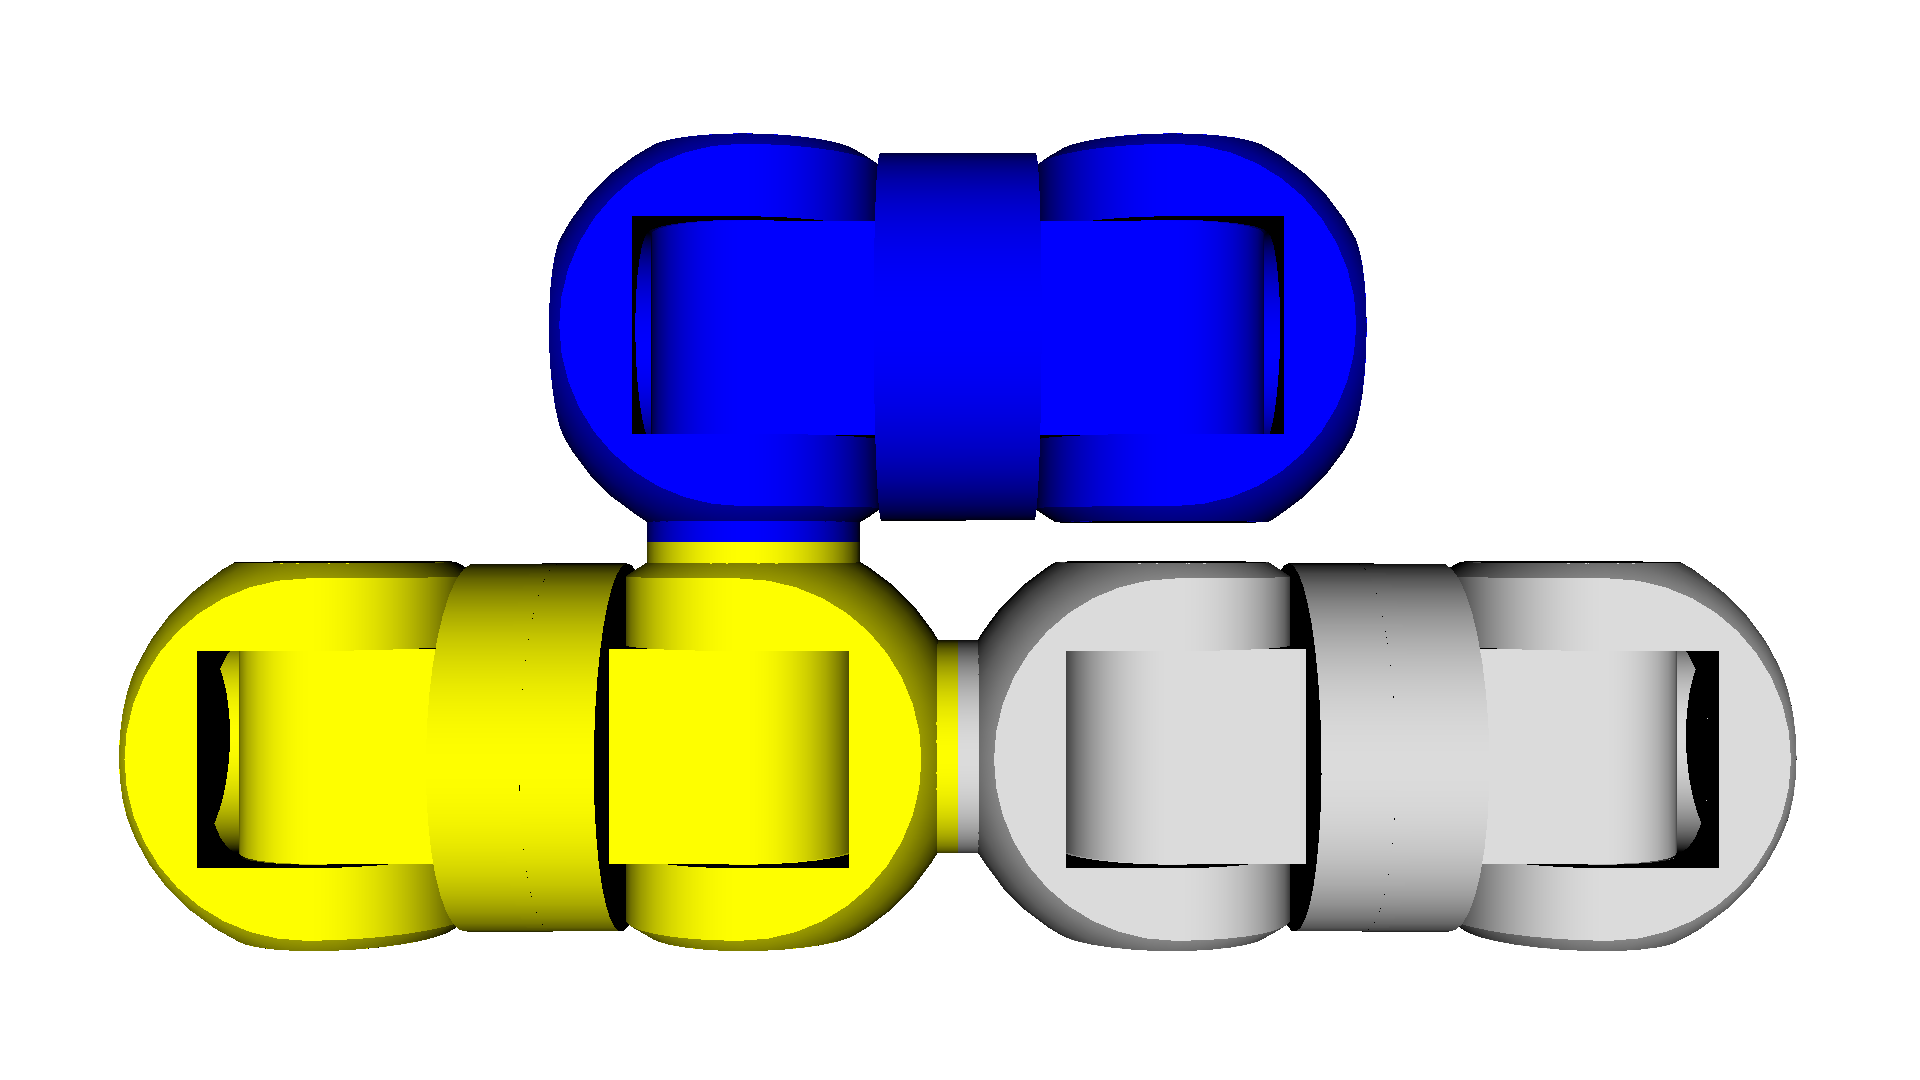
\includegraphics[width=\textwidth]{pictures/connected_rofibot.png}
        \caption[Spojitá konfigurácia.]{Spojitá konfigurácia}
        \label{fig:connectCfg}
    \end{subfigure}
    \begin{subfigure}[b]{0.49\textwidth}
        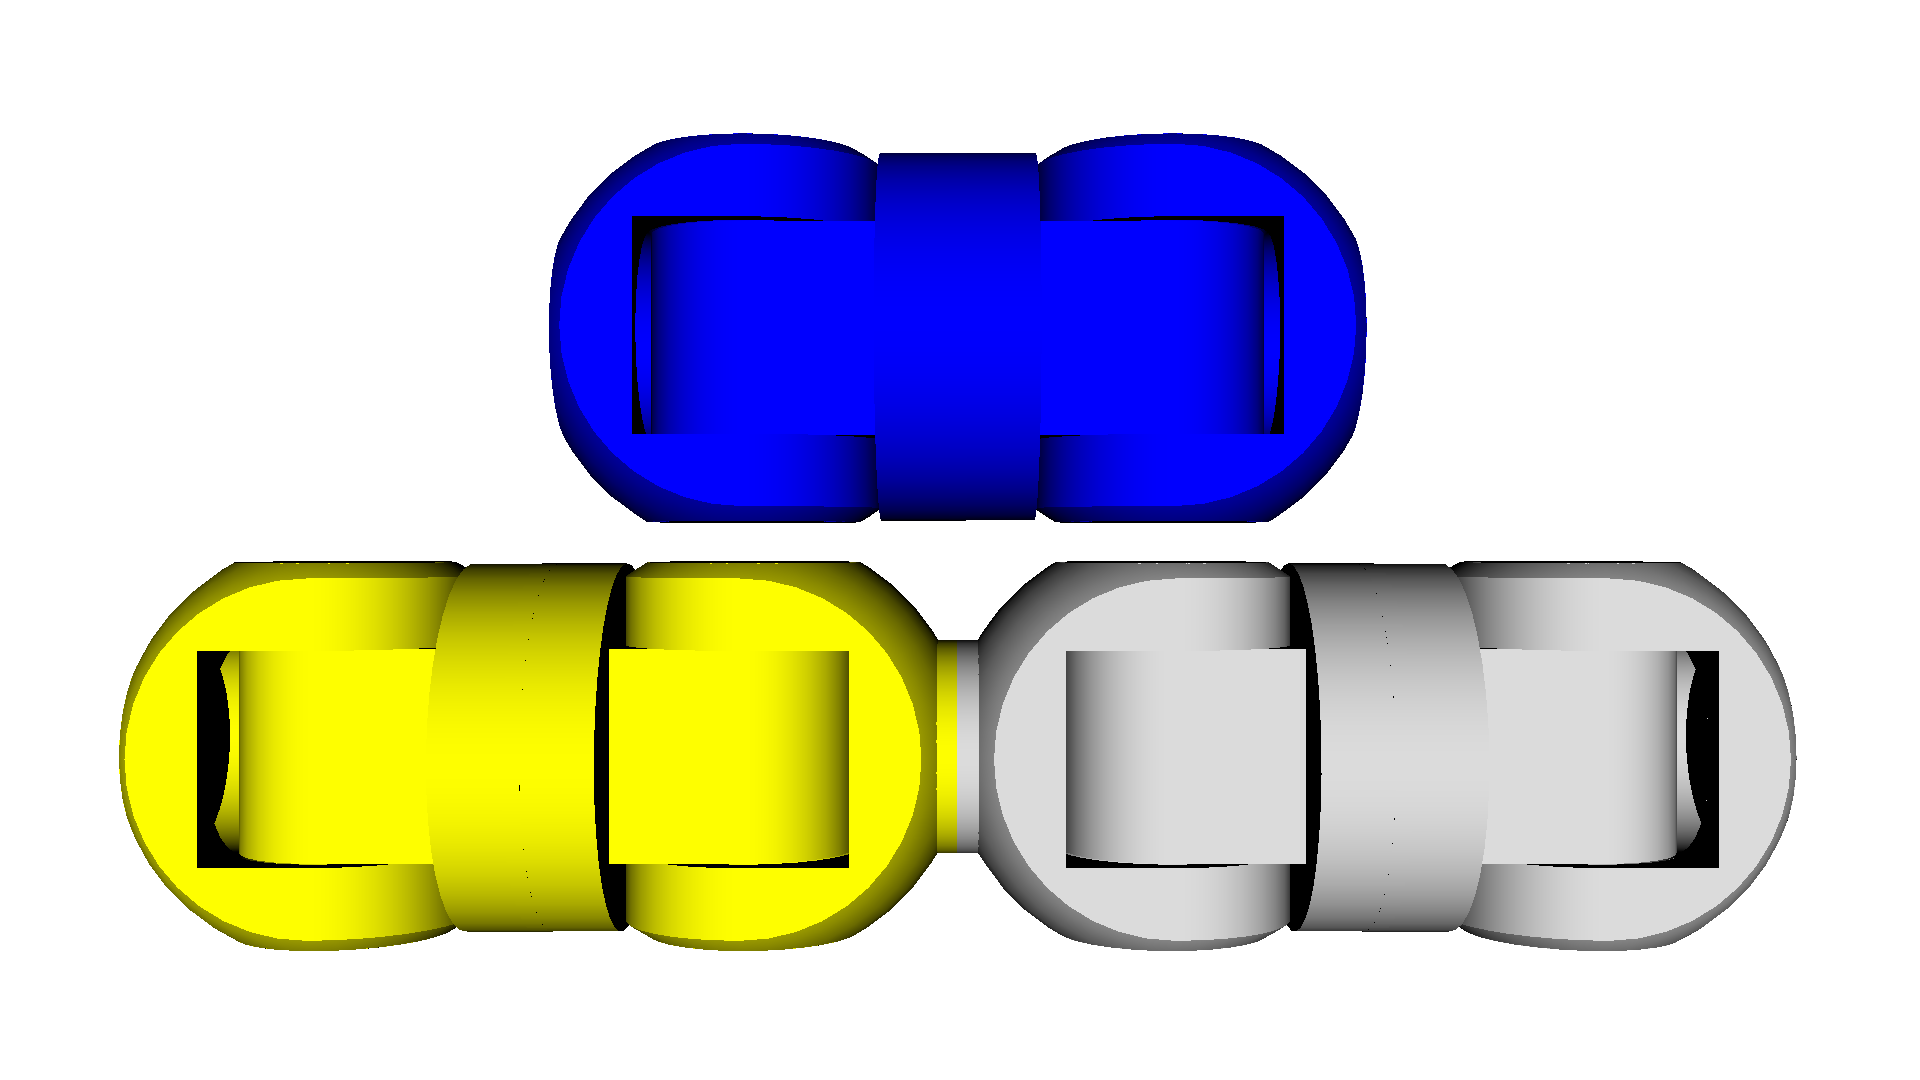
\includegraphics[width=\textwidth]{pictures/disconnected_rofibot.png}
        \caption[Nespojitá konfigurácia.]{Nespojitá konfigurácia}
        \label{fig:disconnectCfg}
    \end{subfigure}
    \caption[Príklad konfigurácie]{Príklad spojitej a nespojitej konfigurácie.}
    \label{fig:exampleCfg}
\end{figure}

Predpokladá sa, že každý modul je definovaný validne. To znamená, že údaje sú z popísaných rozsahov a množín. Každá hrana je definovaná pre oba prepojené moduly, a to v rovnakom tvare. Zároveň platí, že konfigurácia RoFIbota, ktorú popisujú dané stavy modulov, je spojitá a validná. 

\section{Formálna špecifikácia rekonfigurácie RoFIbota}
\label{sec:formalRecfg}
Atomickou zmenou v konfigurácii RoFIbota je \textit{akcia}, ktorá môže byť dvoch druhov. 

Prvým typom akcií je \textit{akcia rotácie}, ktorá sa deje na jednom z modulov RoFIbota a ide o zmenu jedného z parametrov $\alpha$, $\beta$ alebo $\gamma$. Je definovaná nasledovnými parametrami: 
\begin{itemize}
    \item \textit{id} -- \textit{id} modulu, ktorý mení jeden z uhlov; $id \in \mathbb{Z}_0^+$, 
    \item \textit{joint} -- identifikácia stupňa voľnosti; $joint \in \{alfa, beta, gama\}$, 
    \item \textit{angle} -- orientovaný uhol, o ktorý sa daný joint bude otáčať. 
\end{itemize}

Druhý typ akcie je \textit{akcia prepojenia}, ktorá definuje spojenie alebo rozpojenie dvoch modulov. Je definovaná nasledujúcimi parametrami: 
\begin{itemize}
    \item \textit{add} -- príznak, či ide o spojenie alebo rozpojenie,
    \item \textit{edge} -- popis hrany, ktorá buď vznikne alebo zanikne (sedmica definovaná v kapitole \ref{sec:moduleSpec}). 
\end{itemize}

Nie každú akciu je možné aplikovať na akúkoľvek konfiguráciu RoFIbota. \textit{Validná akcia} je akcia, ktorá spĺňa aj nasledujúce podmienky:
\begin{itemize}
    \item akcia rotácie: nesmie dôjsť ku kolízii s inými modulmi (viď obrázok \ref{fig:rotationExample}), 
    \item akcia prepojenia: 
    \begin{itemize}[topsep=-5pt]
        \item oba konektory sa musia podieľať na spojení (príklad na obrázku \ref{fig:reconnectionExample}), 
        \item každý konektor sa podieľa na maximálne jednom spojení,
        \item konektory, ktoré sa majú prepojiť, musia byť fyzicky schopné prepojenia.
    \end{itemize}
\end{itemize}

\begin{figure}[hbt!]
    \centering
    \begin{subfigure}[b]{\textwidth}
        \centering
        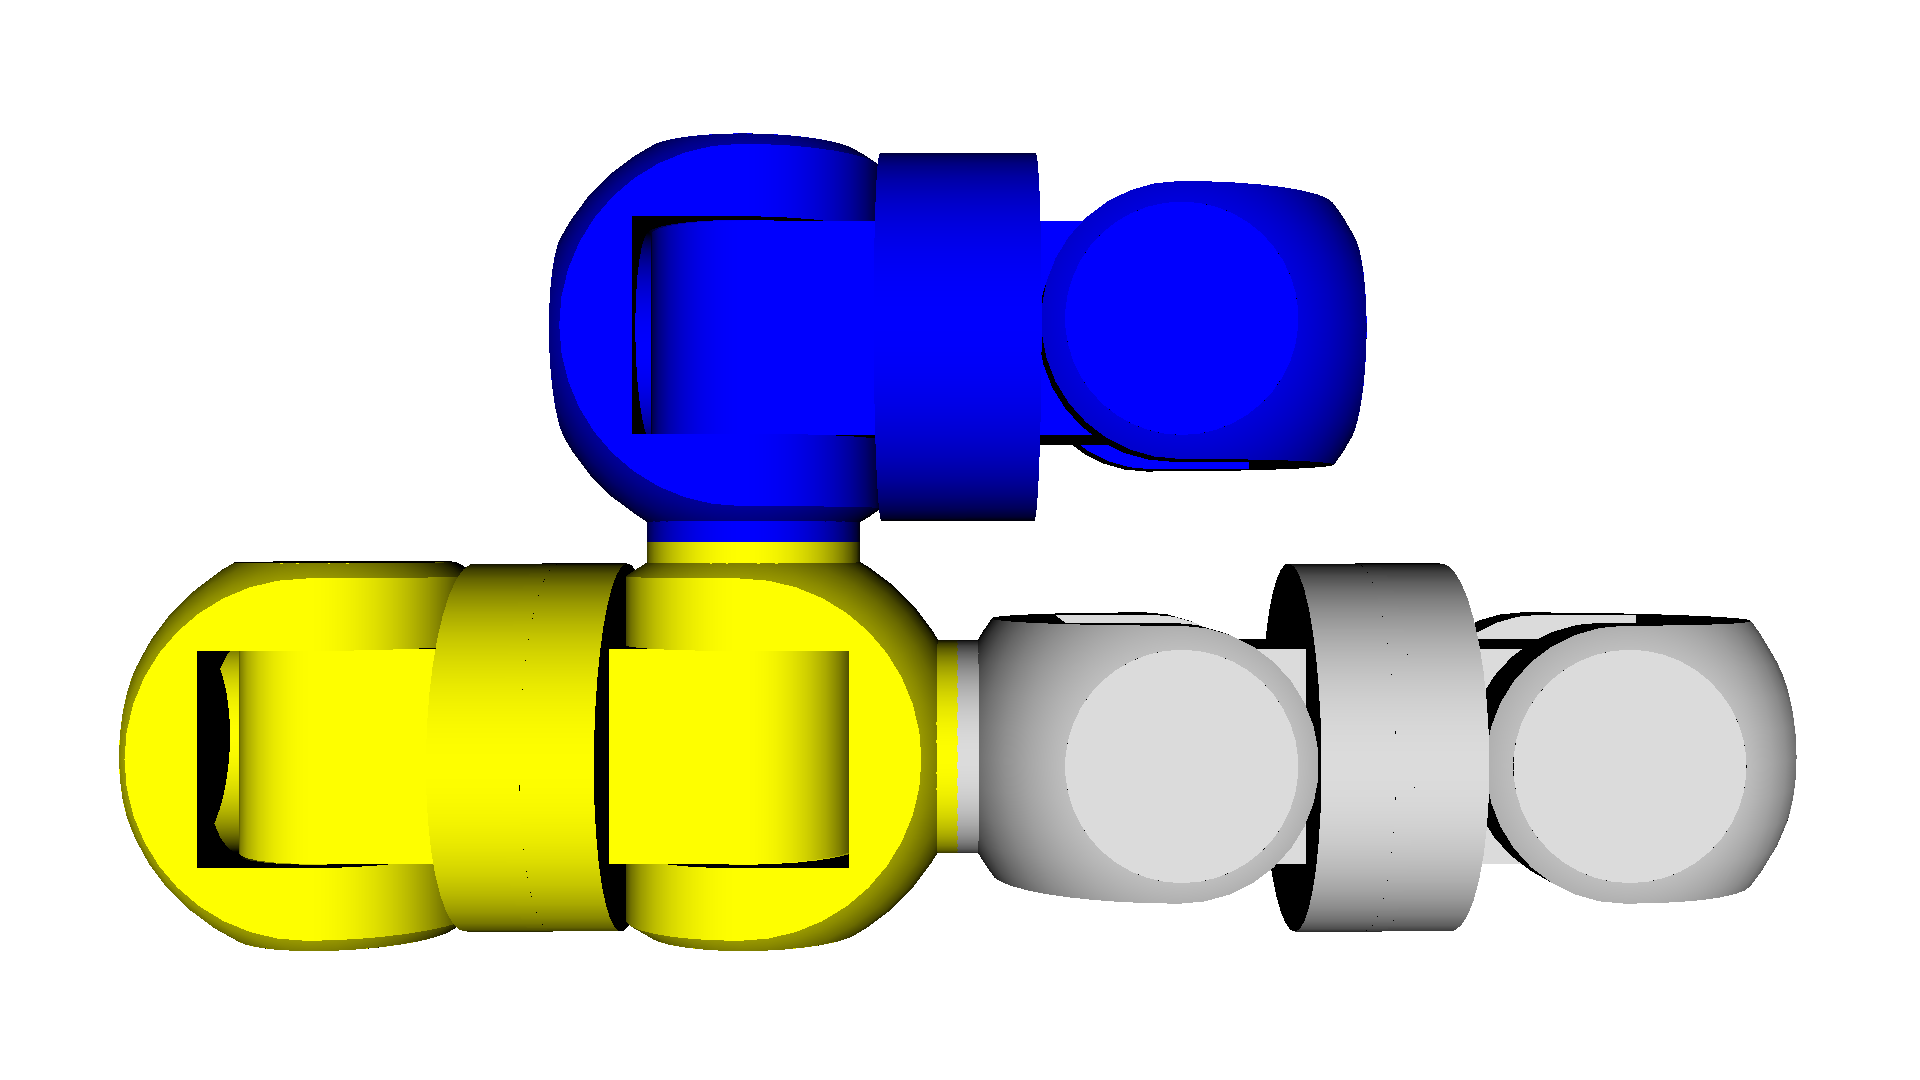
\includegraphics[width=0.47\textwidth]{pictures/rotation_example.png}
        \caption[Pred rotáciou]{Príklad konfigurácie pred rotáciou.}
    \end{subfigure}

    \begin{subfigure}[b]{0.47\textwidth}
        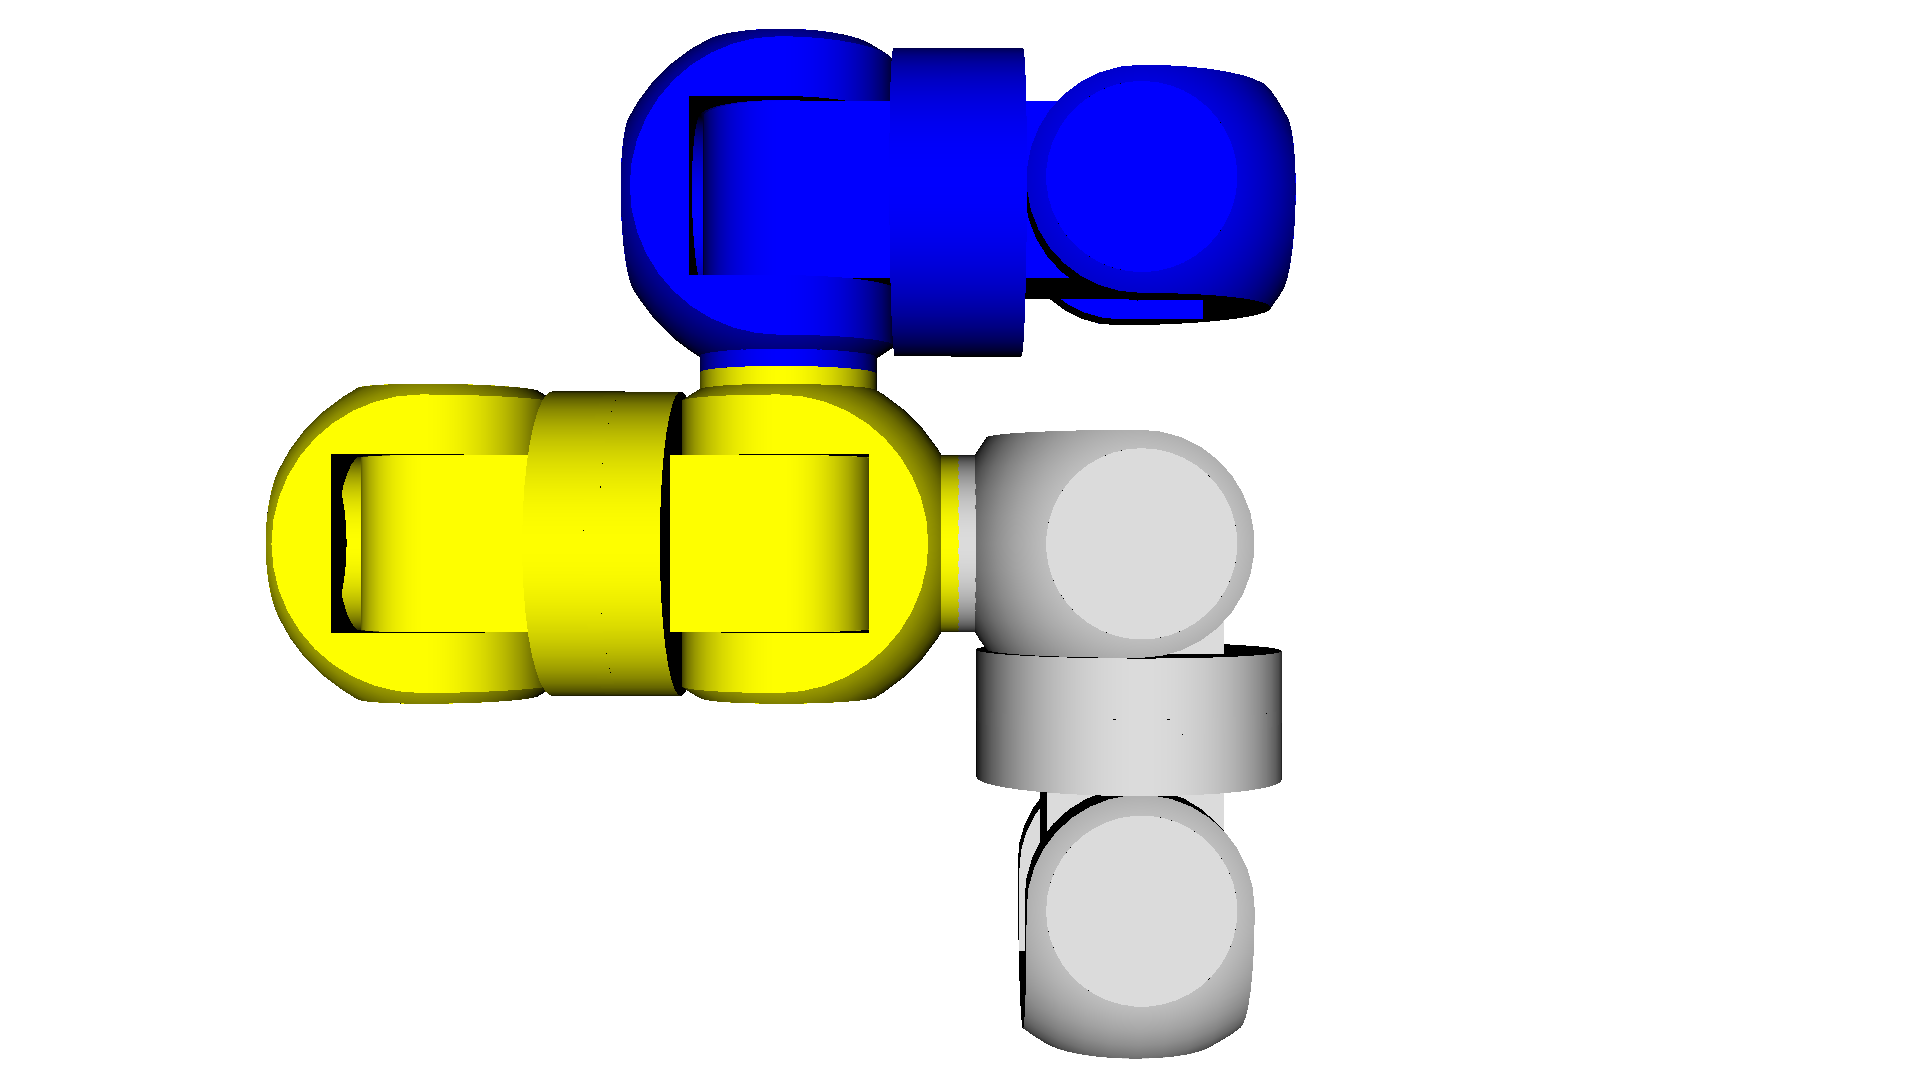
\includegraphics[width=\textwidth]{pictures/rotation_example_correct.png}
        \caption[Validná rotácia]{Validná rotácia modulu.}
    \end{subfigure}
    \begin{subfigure}[b]{0.47\textwidth}
        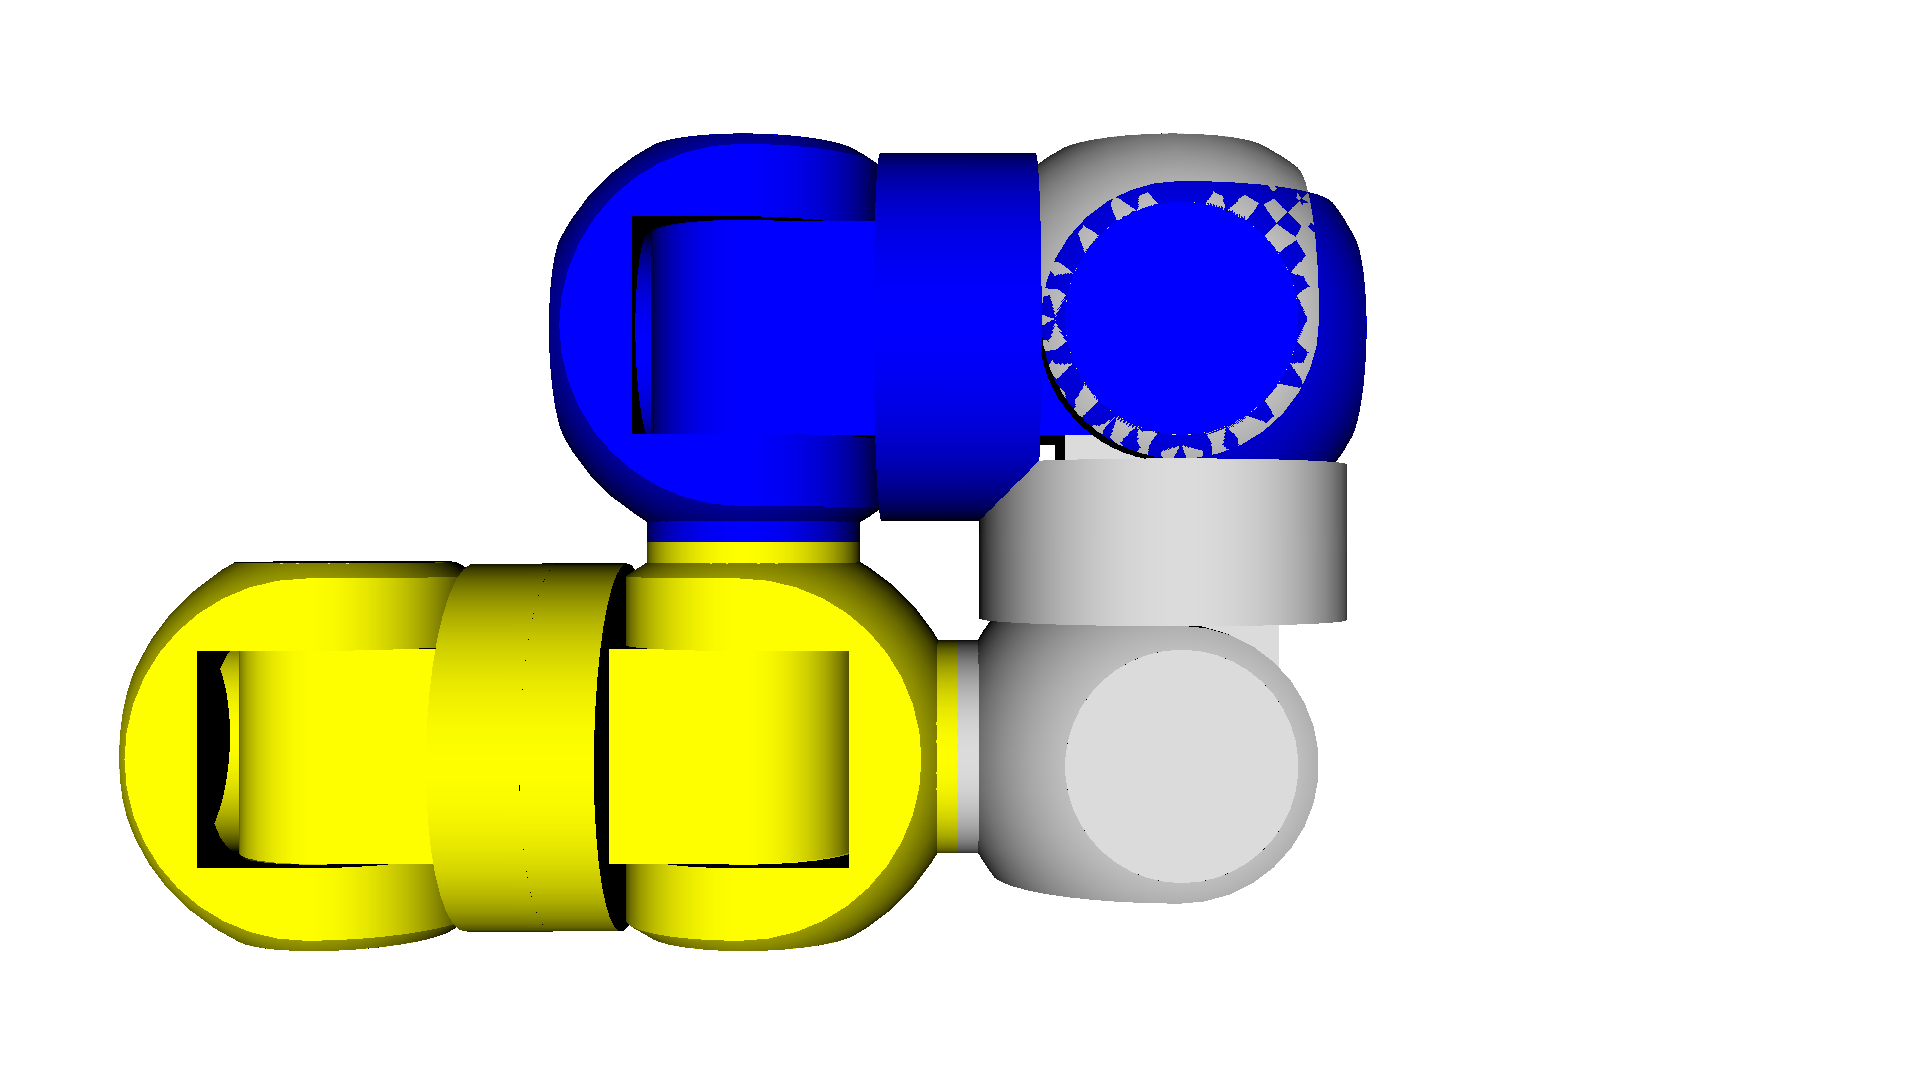
\includegraphics[width=\textwidth]{pictures/rotation_example_wrong.png}
        \caption[Nevalidná rotácia]{Nevalidná rotácia modulu.}
    \end{subfigure}
    \caption[Príklad akcie rotácie]{Príklad akcie rotácie (rotácia bieleho modulu o $90\degree$ uhla $\gamma$).}
    \label{fig:rotationExample}
\end{figure}

\begin{figure}[hbt!]
    \centering
    \begin{subfigure}[b]{\textwidth}
        \centering
        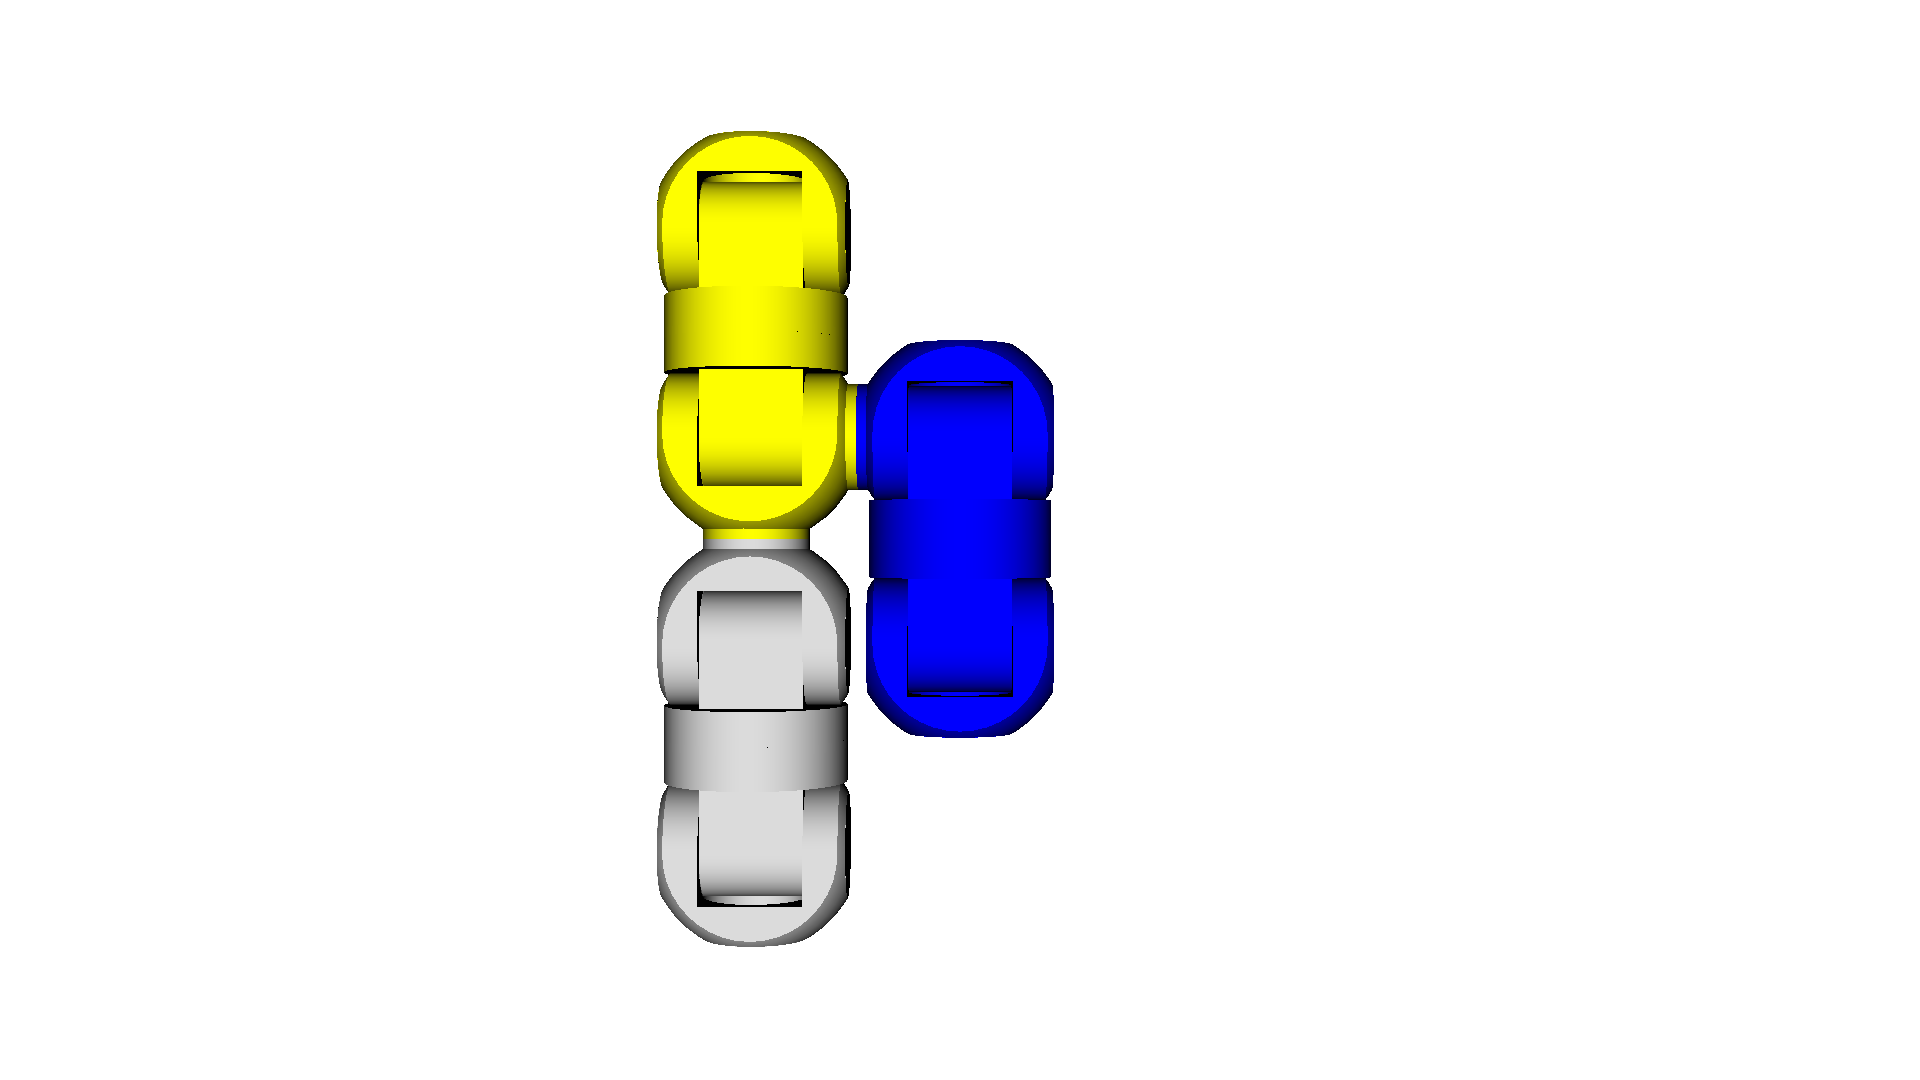
\includegraphics[width=0.8\textwidth]{pictures/reconnection_example.png}
        \caption[Pred prepojením]{Príklad konfigurácie pred vytvorením spojenia.}
    \end{subfigure}

    \begin{subfigure}[b]{0.47\textwidth}
        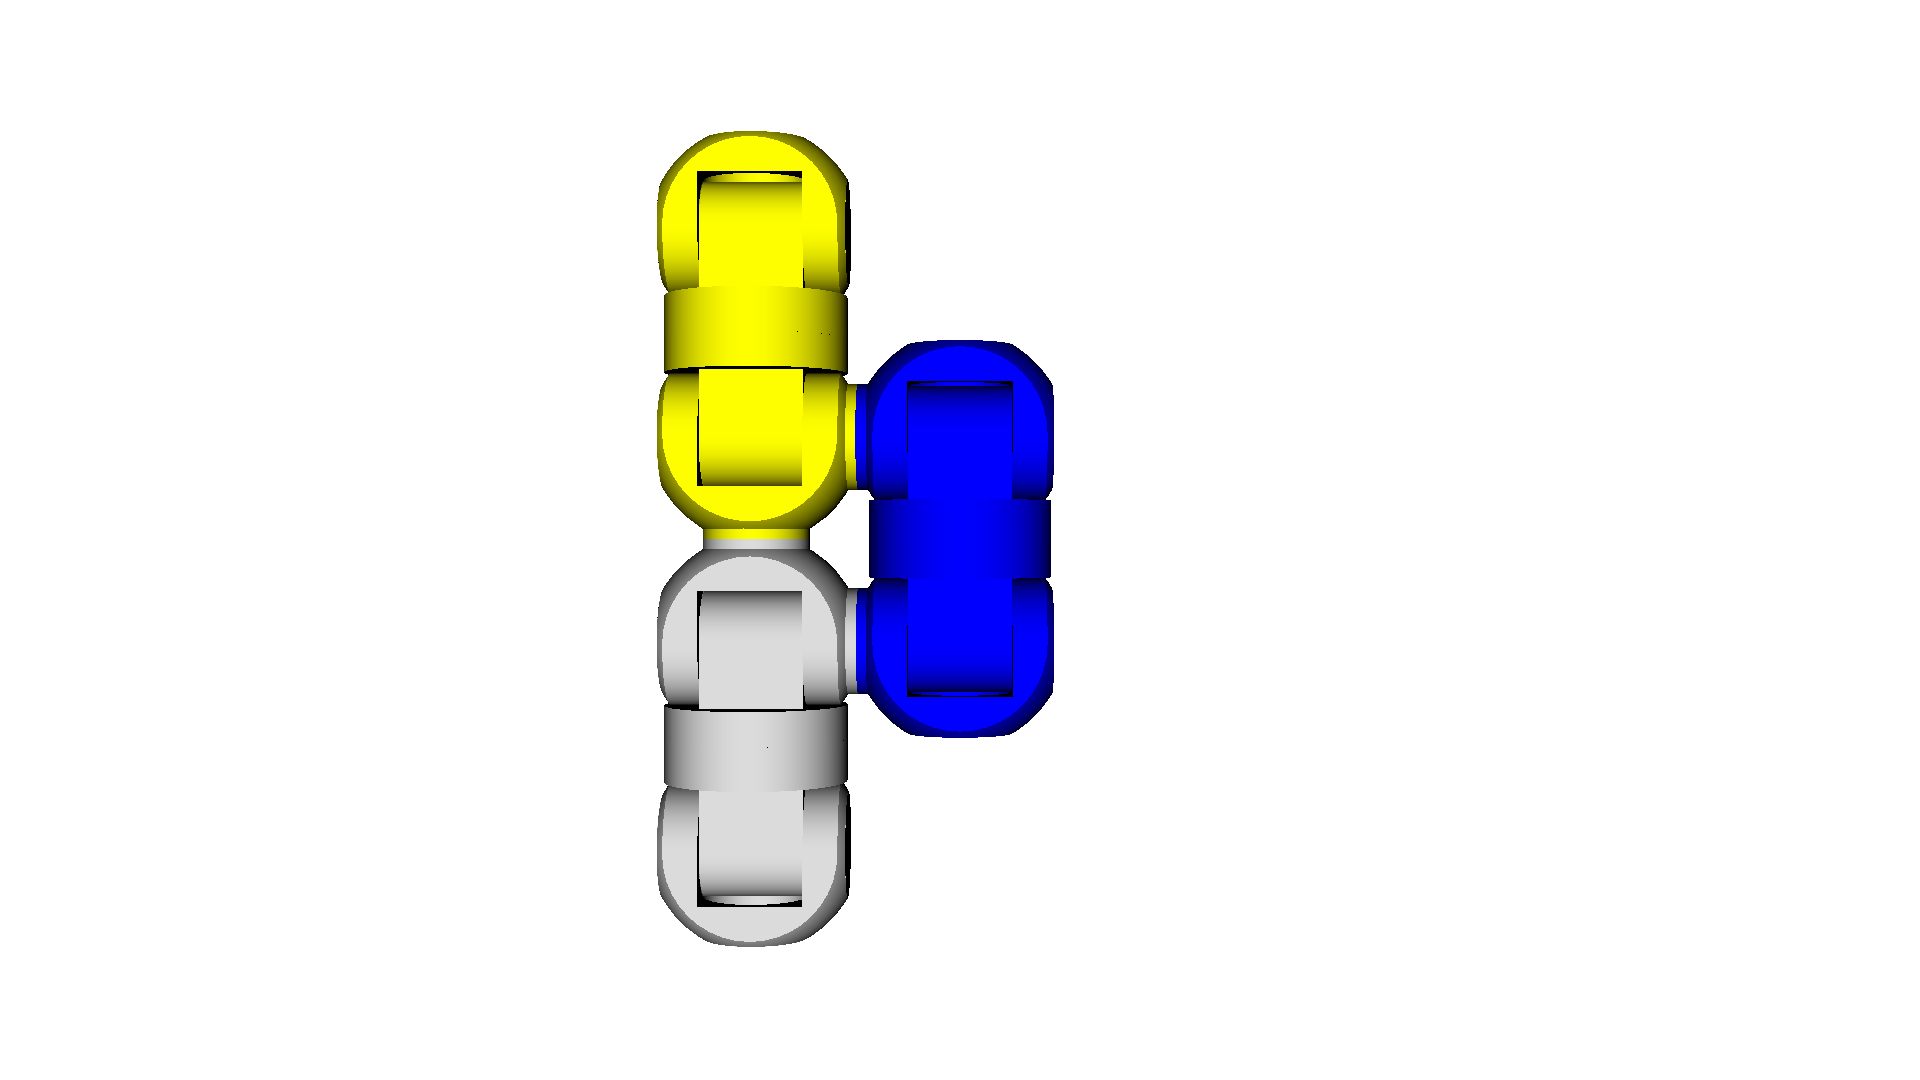
\includegraphics[width=\textwidth]{pictures/reconnection_example_correct.png}
        \caption[Validné spojenie]{Validné spojenie modulov \\(obidva sa podieľajú na spojení).}
    \end{subfigure}
    \begin{subfigure}[b]{0.47\textwidth}
        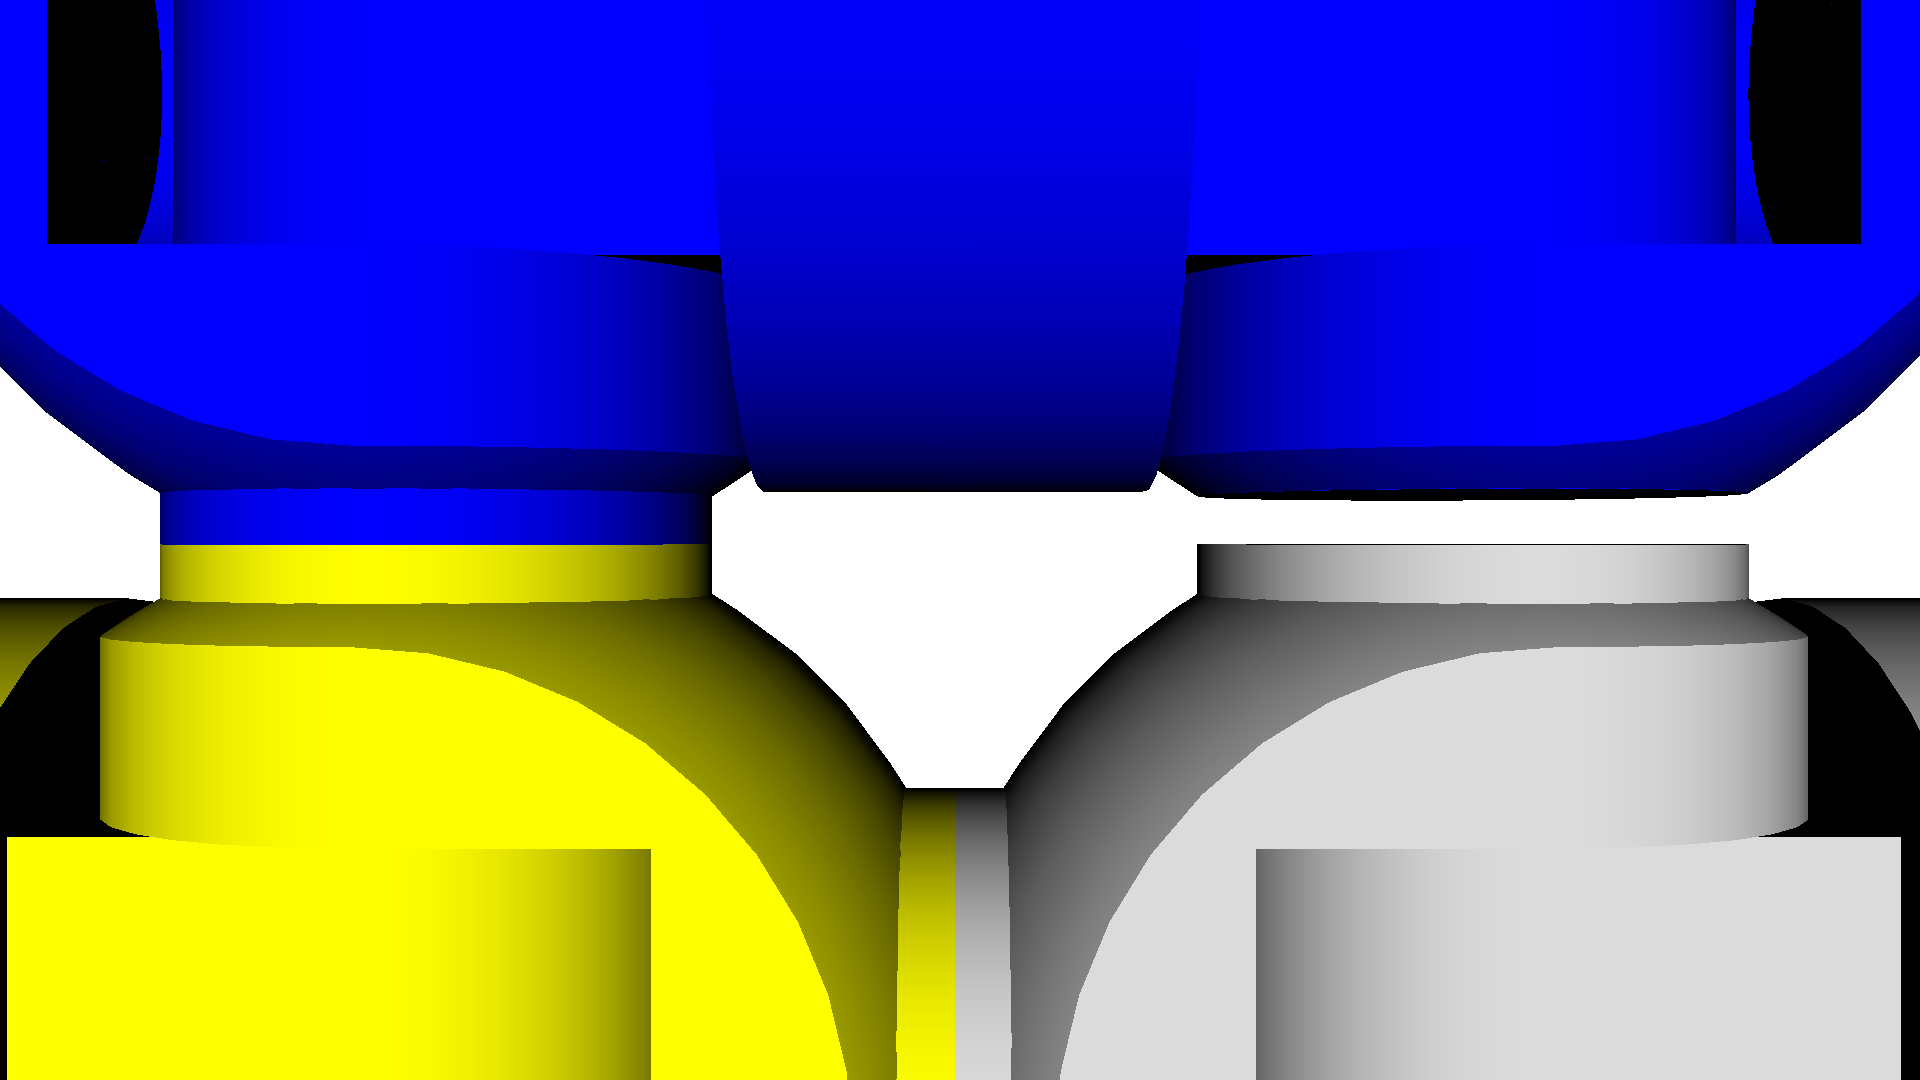
\includegraphics[width=\textwidth]{pictures/reconnection_example_wrong.png}
        \caption[Nevalidné prepojenie]{Nevalidné spojenie modulov \\(modrý sa nepodieľa na spojení).}
    \end{subfigure}
    \caption[Príklad akcie prepojenia]{Príklad akcie prepojenia (medzi bielym a modrým modulom).}
    \label{fig:reconnectionExample}
\end{figure}

% {0, 0, 136},
% {0, 0, 255},
% {119, 119, 255},
% {220, 220, 220},
% {255, 255, 136},
% {255, 255, 0},
% {119, 119, 0}};

\textit{Krok rekonfigurácie} je definovaný ako množina validných akcií. Poradie vykonávania akcií v jednom krku rekonfigurácie nie je presne definované (prebiehajú zároveň, ale synchronizácia nikdy nie je úplne presná). 

Pre spojitých RoFIbotov musí platiť, že ak je konfigurácia pred krokom spojitá a validná, tak aj počas vykonávania kroku a po jeho vykonaní musí byť konfigurácia spojitá a validná. \textit{Validný krok} je krok rekonfigurácie taký, že konfigurácia je spojitá aj v prípade, ak sa vykonajú iba všetky rozpojenia a žiadne iné akcie. 

Rekonfigurácia RoFIbota je definovaná ako postupnosť validných krokov. 

\section{Popis problému}
\label{sec:problemDesc}
Cieľom tejto práce je navrhnúť a implementovať algoritmy na rekonfiguráciu RoFIbotov, ktoré spĺňajú podmienky popísané v tejto kapitole, a následne evaluovať výsledky. 

Diplomová práca \textit{Motion Planning for the RoFI Platform} \cite{vozarovaMasterThesis} popisuje rekonfiguráciu RoFIbotov z centralizovaného pohľadu. To znamená, že algoritmy na rekonfiguráciu majú úplnú znalosť počiatočnej a cieľovej konfigurácie RoFIbota. 

Platforma RoFI je však navrhnutá ako distribuovaný systém, kde najmenšou stavebnou jednotkou je modul. Zároveň je platforma navrhnutá tak, že RoFIbot nemá žiadnu centralizovanú logickú jednotku, ktorá by dokázala riadiť rekonfiguráciu. 

Algoritmy navrhnuté v tejto práci považujú modul za samostatnú entitu, ktorá na vstup dostane počiatočný a cieľový stav modulu, ktorý reprezentuje. Výstupom tejto entity je zoznam akcií, ktoré daný modul vykonal počas rekonfigurácie RoFIbota s prihliadnutím na validitu a spojitosť. V prípade, že sa RoFIbot nedokáže rekonfigurovať z počiatočnej konfigurácie do cieľovej, tak implementované algoritmy túto skutočnosť dokážu identifikovať. 

Samotný modul nepozná celú konfiguráciu RoFIbota (dokonca pri veľkých konfiguráciách by znalosť celej konfigurácie mohla zaberať veľa miesta v pamäti a nebola by potrebná). V tejto práci má každý modul znalosť výhradne o svojom stave, pričom každý ďalší údaj o stave iných modulov vie získať výhradne posielaním si správ so susednými modulmi. 

Implementované algoritmy sú iba simuláciou reálnych rekonfigurácií RoFIbotov, teda nie je nutné striktne dodržiavať všetky fyzikálne zákonitosti reálneho sveta. Tým pádom každý RoFIbot vykonáva svoju rekonfiguráciu „vo vákuu“, bez fyzických obmedzení (ako je napríklad podlaha, či iné prekážky). Pri rekonfigurácii nehrajú rolu ani fyzikálne zákony (napríklad gravitácia). Zároveň musí platiť, že počas celej rekonfigurácie musí byť RoFIbot vo validnej a spojitej konfigurácií. 

To značí, že RoFIbot nemusí mať žiadne vnímanie okolitého sveta. Jedinými prekážkami v pohyboch sú moduly samotné (ich poloha) a tú si entity vedia zistiť pomocou posielania si správ. 

Prínosom tejto práce je simulácia problému rekonfigurácie modulov v distribuovanom prostredí. Súčasťou evaluácie navrhnutých a implementovaných algoritmov je aj porovnanie dĺžky výpočtov a počtu krokov rekonfigurácie distribuovaných algoritmov voči sebe aj voči vybraným algoritmom z diplomovej práce \textit{Motion Planning for the RoFI Platform} \cite{vozarovaMasterThesis}. 

\section{Popis algoritmov na rekonfiguráciu}
\label{sec:algoDesc}
V tejto práci sú navrhnuté a implementovaná dva algoritmy na rekonfiguráciu RoFIbotov, ktoré sa líšia hlavne prístupom k znalosti celej konfigurácie RoFIbota. 

Prvý algoritmus využíva plnú znalosť celej konfigurácie RoFIbota. Zároveň využíva algoritmy na rekonfiguráciu navrhnuté a implementované v diplomovej práci \textit{Motion Planning for the RoFI Platform} \cite{vozarovaMasterThesis}. Výsledok výpočtu rekonfigurácie pomocou motion planning je následne distribuovaný medzi moduly. 

Druhý algoritmus nevyžaduje znalosť celej konfigurácie, ale pomocou zasadenia RoFIbota do súradnicovej sústavy je RoFIbot schopný rekonfigurácie pomocou komunikácie medzi modulmi. 

Pre oba algoritmy platí, že každý modul je reprezentovaný ako samostatná entita, ktorá má na začiatku znalosť o svojom počiatočnom a cieľovom stave. Zároveň má možnosť komunikovať s modulmi, s ktorými je fyzicky prepojený. 

Keďže je táto práca zameraná na samotné algoritmy rekonfigurácie, tak môžeme predpokladať, že moduly dokážu komunikovať každý s každým, nakoľko je RoFIbot v každom momente rekonfigurácie spojitý. Problém posielania správ rieši nižšia softvérová vrstva, ktorá je už vo fyzických moduloch implementovaná a je možné ju využívať. 

\subsection{Algoritmus s úplnou znalosťou konfigurácie}
\label{sec:motionPlanningAlgo}
V počiatočnej fáze algoritmu pošle každý z modulov svoju počiatočnú a cieľovú konfiguráciu pomocou broadcastu. Tým zároveň každý modul získa stavy ostatných modulov RoFIbota. Broadcast funguje iba na spojitej časti RoFIbota a je vo fyzických moduloch implementovaný na nižšej úrovni softvéru.

Aby mal modul úplnú konfiguráciu RoFIbota, je nutné získať hodnoty stupňov voľnosti $\alpha$, $\beta$ a $\gamma$ od všetkých modulov RoFIbota a zároveň je nutné mať plnú informáciu o všetkých prepojeniach modulov. Všetky tieto údaje sú uložené v stavoch modulov. Z toho vyplýva, že po vzájomnom zdieľaní stavov medzi modulmi je každý modul schopný reprezentovať celú počiatočnú aj cieľovú konfiguráciu RoFIbota. To znamená, že každý modul je schopný vypočítať celú rekonfiguráciu pomocou algoritmov implementovaných v diplomovej práci \textit{Motion Planning for the RoFI Platform} \cite{vozarovaMasterThesis}, teda postupnosť validných krokov. 

Cieľom je, aby každý modul vypočítal rovnakú postupnosť krokov. To znamená, že z algoritmov implementovaných v spomínanej diplomovej práci je nutné vybrať deterministický algoritmus, ktorým je buď \textit{BFS} alebo \textit{A*} (algoritmus \textit{RRT} nie je deterministický). Výsledky porovnania týchto dvoch algoritmov v spomínanej diplomovej práci ukazujú, že algoritmus \textit{A*} je časovo rýchlejší ako algoritmus \textit{BFS}. Z tohto dôvodu budú moduly využívať algoritmus \textit{A*}. 

Pre algoritmus \textit{A*} je nutné vybrať heuristiku (pre každý modul rovnakú). Pre účely tejto práce bola vybraná heuristika, ktorá počíta rozdiel v hodnotách všetkých uhlov voľnosti. Zároveň budú moduly počítať postupnosť krokov tak, aby sa v každom kroku udiala výhradne jedna validná akcia. Algoritmus \textit{A*} je implementovaný tak, aby bolo možné nastaviť limit na maximálny počet akcií, ktoré je možné vykonať v jednom kroku rekonfigurácie. Obmedzenie na jednu akciu v kroku je vhodné hlavne kvôli optimalizácii krokov rekonfigurácie, ktorá je popísaná neskôr. 

Po výpočte má každý modul napočítanú tú istú postupnosť krokov, ktoré sa majú vykonávať na to, aby sa RoFIbot mohol rekonfigurovať, alebo dokáže identifikovať, že rekonfigurácia nie je možná. 

Ak nie je rekonfigurácia možná, tak tento fakt identifikuje už výpočet algoritmu \textit{A*}. Tým pádom aj výpočet algoritmu navrhnutého pre túto prácu dokáže túto skutočnosť identifikovať a vo výpočte už ďalej nepokračuje. 

Ak je rekonfigurácia validná, tak následne budú moduly túto postupnosť optimalizovať. Optimalizácia je vhodná hlavne z dôvodu zrýchlenia fyzickej rekonfigurácie RoFIbota, čiže chceme, aby sa viacero krokov pôvodnej postupnosti vykonávalo v rovnakom čase. 

Optimalizácia bude opäť iba heuristikou a nezaručuje nájdenie optimálneho riešenia (vzhľadom na počet krokov rekonfigurácie) paralelizácie krokov, ale zaručuje, že nájdené riešenie ostane validnou rekonfiguráciou RoFIbota. Táto optimalizácia spočíva v dvoch fázach, a to v spájaní krokov a v ich výmenách. Tieto optimalizácie je možné robiť výhradne na dvoch krokoch, ktoré po sebe nasledujú. 

Navrhnutá optimalizácia intuitívne prebieha tak, že pospája čo najviac krokov dohromady a následne sa novovzniknuté kroky pokúsi povymieňať, aby bola postupnosť krokov rekonfigurácie naďalej validná. Toto sa opakuje, až kým sa vo fáze spájania nevykoná žiadna zmena. 

Z formálneho hľadiska ide o tieto algoritmy. Pre lepšiu orientáciu si zadefinujme $\mathcal{C}_i$ ako konfiguráciu RoFIbota po $i$-tom kroku. Teda $\mathcal{C}_0$ je počiatočná konfigurácia. Ďalej si definujme $\mathcal{S}_i$ ako $i$-ty krok rekonfigurácie. Zároveň, nech je operátor \lstinline{<*>} definovaný ako aplikácia kroku $\mathcal{S}$ na konfiguráciu $\mathcal{C}$, teda platí $\mathcal{S}_{i + 1}$ \lstinline{<*>} $\mathcal{C}_i = \mathcal{C}_{i + 1}$. Nech $\mathcal{S}'_i$ je zjednotenie akcií v krokoch $\mathcal{S}_i$ a $\mathcal{S}_{i + 1}$. 

\textit{Spojenie krokov} $\mathcal{S}_i$ a $\mathcal{S}_{i + 1}$ je možné iba v prípade ak platí, že $\mathcal{S}'_i$ je validný krok. Zároveň musí platiť, že ak zjednotenie krokov $\mathcal{S}_i$ a $\mathcal{S}_{i + 1}$ aplikujeme na konfiguráciu $\mathcal{C}_{i - 1}$, tak výsledok bude rovnaký, ako keby sme ich aplikovali postupne. To je ekvivalentne zapísané nasledovne: 
\begin{align}
\label{align:stepJoin}
\mathcal{S}_{i + 1} \lstinline{<*>} (\mathcal{S}_i \lstinline{<*>} \mathcal{C}_{i - 1}) = \mathcal{S}'_i \lstinline{<*>} \mathcal{C}_{i - 1}. 
\end{align}

Rovnosť \ref{align:stepJoin} však popisuje iba spojenie dvoch krokov. Navrhnutý algoritmus sa snaží minimalizovať počet krokov celkovo, a teda je potrebné systematicky spájať viaceré kroky. 

Toto spájanie prebieha nasledovne: Postupne sa prechádza každý index krokov od $1$ až po predposledný krok rekonfigurácie. Ak sa kroky $\mathcal{S}_i$ a $\mathcal{S}_{i + 1}$ dajú spojiť, tak sa postupnosť upraví tak, že tieto dva kroky sa vymažú, na ich miesto sa vloží $\mathcal{S}'_i$ (ostatné kroky sa následne prečíslujú) a pokračuje sa opäť testovaním spájania krokov na indexoch $i$ (novovytvorený krok $\mathcal{S}'_i$) a $i + 1$. Tento postup je popísaný aj v algoritme~\ref{algorithm:stepJoin}. 

\begin{algorithm}
    \caption{joinSteps}
    \label{algorithm:stepJoin}
    \DontPrintSemicolon
    \SetKwInOut{Input}{vstup}\SetKwInOut{Output}{výstup}
    \SetKwData{CurrIndex}{i}
    \SetKwData{NextIndex}{\CurrIndex + 1}
    \SetKwData{JoinStep}{$\mathcal{S}'$}
    \SetKwData{Cfg}{$\mathcal{C}_{\CurrIndex - 1}$}
    \SetKwData{Steps}{stepVector}
    \Input{\ \Steps\ -- postupnosť krokov rekonfigurácie.}
    \Output{\ \Steps\ -- postupnosť krokov rekonfigurácie taká, že žiadne dva susedné kroky sa už nedajú spojiť.}
    
    \CurrIndex $\leftarrow$ 1\;
    \While{\CurrIndex < $|\Steps|$}{
        \JoinStep $\leftarrow \mathcal{S}_\CurrIndex$ $\cup$ $\mathcal{S}_\NextIndex$\;
        
        \eIf{\upshape $\mathcal{S}_\NextIndex$ \lstinline{<*>} ($\mathcal{S}_\CurrIndex$ \lstinline{<*>} \Cfg) $=$ \JoinStep \lstinline{<*>} \Cfg\ {\bf and} \JoinStep \textit{je validný}}{
            vymaž $\mathcal{S}_\NextIndex$ a $\mathcal{S}_\CurrIndex$\;
            na index \CurrIndex vlož krok \JoinStep\;
        }{
            \CurrIndex $\leftarrow$ \NextIndex\;
        }
    }
\end{algorithm}

\textit{Výmena krokov} $\mathcal{S}_i$ a $\mathcal{S}_{i + 1}$ je definovaná tak, že sa vymení poradie týchto dvoch krokov. Táto výmena musí spĺňať nasledujúce podmienky: Ak sa najskôr vykoná krok $\mathcal{S}_{i + 1}$, a až potom krok $\mathcal{S}_i$, tak bude výsledok rovnaký ako pri vykonaní krokov v pôvodnom poradí. Zároveň však musí platiť, že aj vymenené poradie krokov je validné a dodržiavajú sa podmienky na validný krok (napr. spojitosť RoFIbota). Formálne je prvá podmienka definovaná nasledovne: 
\begin{align}
\label{align:stepSwap}
\mathcal{S}_{i + 1} \lstinline{<*>} (\mathcal{S}_i \lstinline{<*>} \mathcal{C}_{i - 1}) = \mathcal{S}_i \lstinline{<*>} (\mathcal{S}_{i + 1} \lstinline{<*>} \mathcal{C}_{i - 1}). 
\end{align}

Rovnosť \ref{align:stepSwap} popisuje iba výmenu dvoch krokov. Cieľom algoritmu bude však v časti výmeny krokov vymeniť ich viacero, nakoľko tieto výmeny môžu umožniť ďalšie spájania krokov. 

Tieto výmeny prebiehajú nasledovne: Postupne sa prechádza každý index krokov od $1$ až po predposledný krok rekonfigurácie. Ak sa kroky $\mathcal{S}_i$ a $\mathcal{S}_{i + 1}$ dajú vymeniť, tak sa vymenia. Následne sa pokračuje testovaním výmeny pre krok na indexe $i + 1$. Tento postup je uvedený pomocou pseudokódu v algoritme~\ref{algorithm:stepSwap}. 

\begin{algorithm}
    \caption{swapSteps}
    \label{algorithm:stepSwap}
    
    \DontPrintSemicolon
    \SetKwInOut{Input}{vstup}\SetKwInOut{Output}{výstup}
    \SetKwData{CurrIndex}{i}
    \SetKwData{NextIndex}{\CurrIndex + 1}
    \SetKwData{Steps}{stepVector}
    \SetKwData{Cfg}{$\mathcal{C}_{\CurrIndex - 1}$}
    \Input{\ \Steps\ -- postupnosť krokov rekonfigurácie.}
    \Output{\ \Steps\ -- postupnosť krokov rekonfigurácie po výmene krokov.}
    
    \For{\CurrIndex $\leftarrow 1$ \KwTo $|\Steps|$}{
        \If{\upshape $\mathcal{S}_\CurrIndex$ \lstinline{<*>} ($\mathcal{S}_\NextIndex$ \lstinline{<*>} \Cfg) $=$ $\mathcal{S}_\NextIndex$ \lstinline{<*>} ($\mathcal{S}_\CurrIndex$ \lstinline{<*>} \Cfg) \\ \hspace{12}{\bf and} $\mathcal{S}_\NextIndex$ a $\mathcal{S}_\CurrIndex$ \textit{validné v tomto poradí}}{
            vymeň $\mathcal{S}_\CurrIndex$ a $\mathcal{S}_\NextIndex$\;
        }
    }
\end{algorithm}

Celá optimalizácia prebieha nasledovným spôsobom: V prvom rade sa vykoná spájanie krokov. Následne opakuje výmena krokov a spájanie krokov, a to dovtedy kým spájanie krokov vykoná nejakú zmenu. Táto optimalizácia je znázornená aj v algoritme~\ref{algorithm:algo1}. 

\begin{algorithm}
    \caption{Optimalizácia krokov rekonfigurácie. }
    \label{algorithm:algo1}
    
    \DontPrintSemicolon
    \SetKwInOut{Input}{vstup}\SetKwInOut{Output}{výstup}
    \SetKwData{Steps}{stepVector}
    \SetKwRepeat{Do}{do}{while}
    \Input{\ \Steps\ -- postupnosť krokov na optimalizáciu.}
    \Output{\ \Steps\ -- optimalizovaná postupnosť krokov.}
    
    \Steps $\leftarrow$ joinSteps(\Steps)\;
    \Do{\Steps sa zmenil po spojení krokov}{
        \Steps $\leftarrow$ swapSteps(\Steps)\;
        \Steps $\leftarrow$ joinSteps(\Steps)\;
    }
\end{algorithm}

Vyššie popísaná optimalizácia vždy zastaví. Algoritmus \ref{algorithm:stepJoin} po každom cykle buď zvýši hodnotu aktuálneho indexu, alebo zníži celkový počet krokov, teda v každom prípade sa zníži hodnota rozdielu medzi celkovým počtom krokov a aktuálnym indexom. To znamená, že v konečnom čase sa dostane na hodnotu menšiu ako $1$, teda cyklus skončí. V algoritme \ref{algorithm:stepSwap} je využitý cyklus $for$, ktorý zaručene skončí v konečnom čase. 

Ostáva dokázať, že algoritmus \ref{algorithm:algo1} skončí. Cyklus je podmienený výhradne tým, či nastane zmena po spájaní krokov. Každým prechodom cyklu vieme, že sa počet krokov určite zmenšil (nastalo aspoň jedno spojenie), takže v konečnom čase sa buď spojenie neuskutoční alebo bude počet krokov rovný $1$, čo bude znamenať, že v nasledujúcom kroku sa nebude môcť vykonať spojenie krokov, čím sa ukončí cyklus. 

Táto optimalizácia je korektná, nakoľko sa vykonávajú iba korektné akcie spojenia a výmeny, ktoré sa vždy kontrolujú pred ich vykonaním. Preto ak optimalizácia dostane na vstup korektnú postupnosť krokov, tak na výstup vráti optimalizovanú korektnú postupnosť krokov. 

Každý modul teda optimalizoval vypočítanú postupnosť krokov rekonfigurácie. Nakoľko je každý algoritmus deterministický, tak každý z nich vypočíta rovnaký výsledok. Tým pádom sa môže začať fyzická rekonfigurácia, ktorá je daná postupnosťou krokov, teda každý modul vie, v ktorom čase má vykonať akú zmenu. 

Moduly vzájomne komunikujú a posielajú si informácie, že už vykonali daný krok a môže nastať ďalší. Prvý krok môže nastať hneď ako každý dopočíta optimalizáciu. Ak modul vykoná fyzickú akciu v $i$-tom kroku, tak pošle správu každému modulu v $(i + 1)$-tom kroku, že daný modul už vykonal $i$-ty krok. Modul začne vykonávať fyzickú akciu v $(i + 1)$-tom kroku až v prípade, ak dostal správu od každého modulu, ktorý mal vykonávať akciu v $i$-tom kroku. Ak má modul vykonávať viacero akcií v jednom kroku, tak správy posiela až po vykonaní všetkých akcií. Po vykonaní akcií v poslednom kroku rekonfigurácie sa správy už neposielajú. 

Tento algoritmus je navrhnutý tak, že ak niektorý z modulov z nejakého dôvodu nie je schopný výpočtov, tak je možné mu výsledky iba poslať. Zároveň je navrhnutý tak, aby sa dal ľahko adaptovať na zmeny a vylepšenia, pričom niektoré sú popísané v kapitole \ref{sec:future}.  

\subsection{Distribuovaný algoritmus}
\label{sec:distributedAlgo}
Druhý implementovaný algoritmus nepotrebuje znalosť celej konfigurácie RoFIbota. Z intuitívneho pohľadu algoritmus spočíva v tom, že sa v každom kroku vyberie modul, ktorý sa pokúsi priblížiť svoj stav bližšie k cieľovému stavu. Pod pojmom priblížiť sa rozumie buď otočenie niektorým zo stupňov voľnosti, odpojenie niektorej z aktuálnych hrán, ktoré v koncovom stave nie sú, alebo pripojenie k inému modulu tak, aby tvorili hranu, ktorá je v koncovom stave modulu. Nakoľko je RoFIbot vsadený do 3D mriežky, tak v tomto algoritme používame súradnicový systém s predpokladom, že veľkosť hrany mriežky je $1$\,cm. 

Spôsob zavedenia súradnicového systému a aj algoritmus na výpočet súradníc pre ostatné moduly sú prevzaté z diplomovej práce \textit{Motion Planning for the RoFI Platform} \cite{vozarovaMasterThesis}. Základom je definovanie osí súradnicového systému, ktoré sú určené podľa strany A modulu s najnižším \textit{id}, tak ako je to zobrazené na obrázku \ref{fig:moduleAxis}. 

\begin{figure}[hbt!]
    \centering
    \begin{subfigure}[b]{0.47\textwidth}
        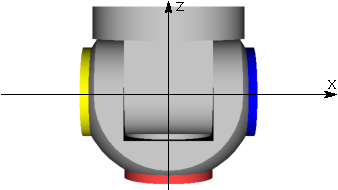
\includegraphics[width=\textwidth]{pictures/module_dock_identification.pdf}
        \caption[Pohľad spredu]{Pohľad spredu.}
    \end{subfigure}
    \begin{subfigure}[b]{0.47\textwidth}
        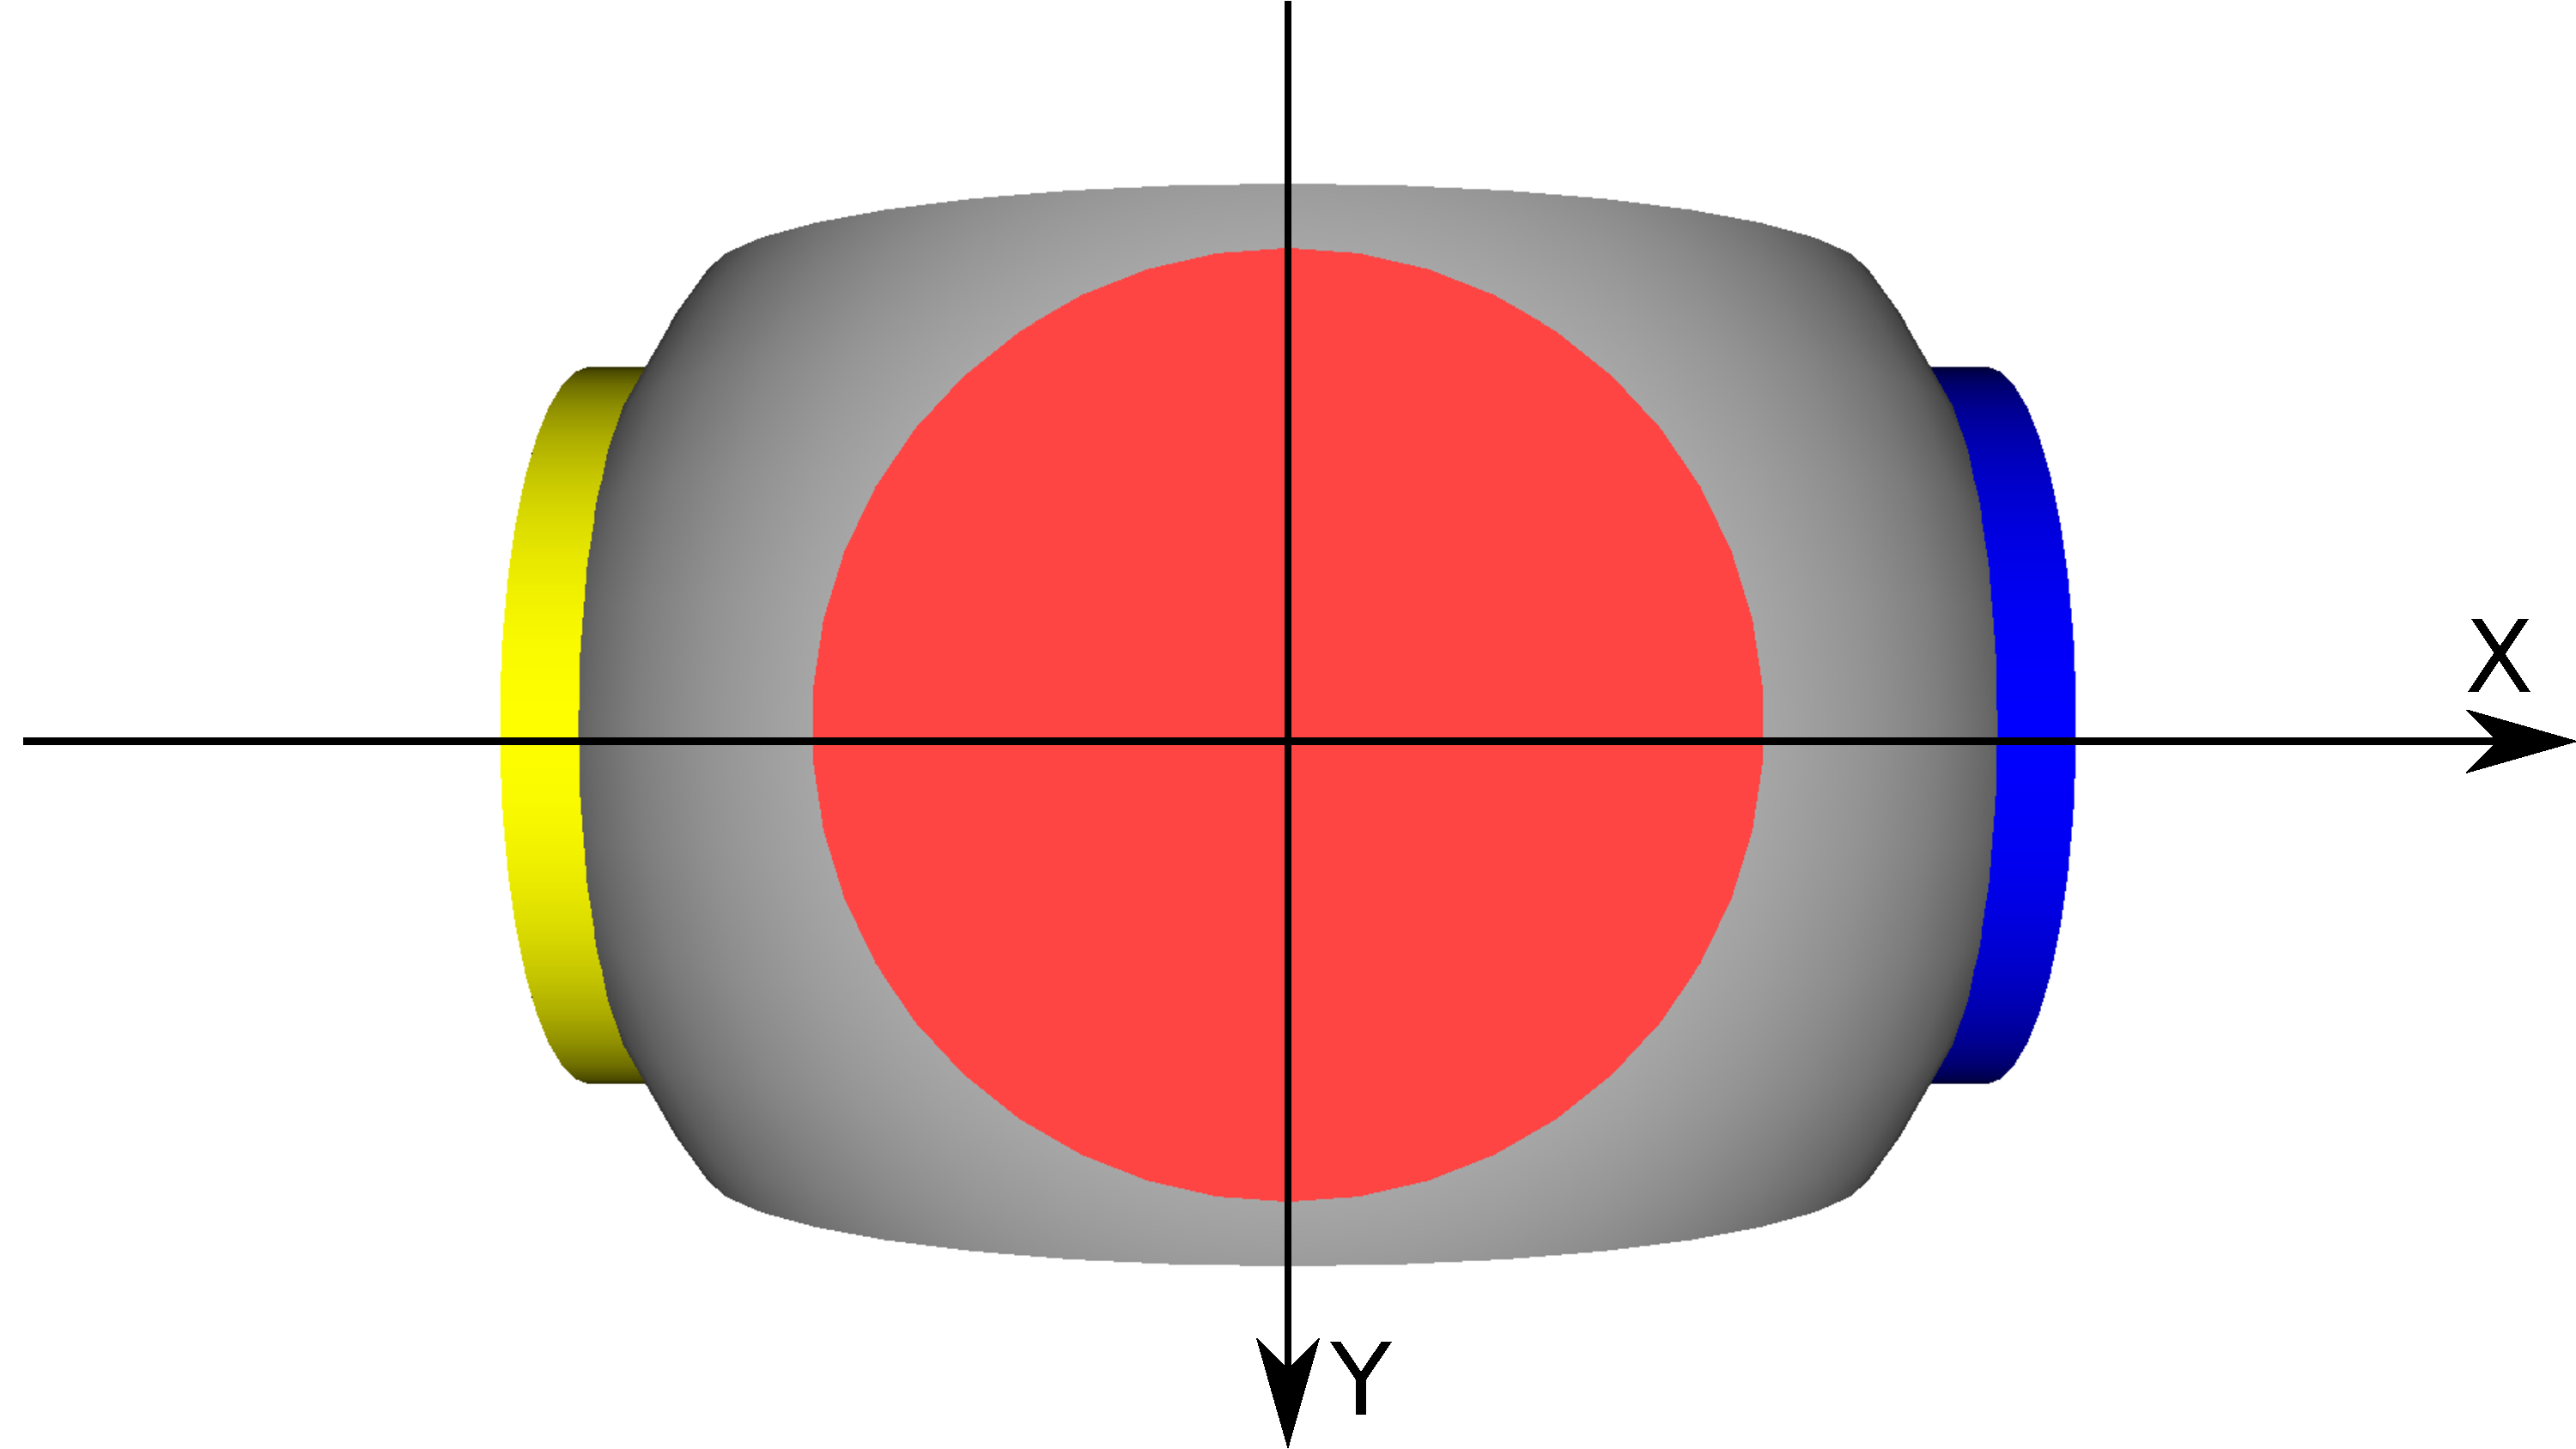
\includegraphics[width=\textwidth]{pictures/module_dock_identification_bottom.pdf}
        \caption[Pohľad zospodu]{Pohľad zospodu.}
    \end{subfigure}
    \caption[Definícia osí súradnicového systému]{Definícia osí súradnicového systému podľa polohy konektorov \textcolor{white}{\colorbox{modra}{$X+$}}, \colorbox{zlta}{$X-$} a \colorbox{cervena}{$Z-$} strany A v základnej pozícii. Ide o pravotočivý súradnicový systém. }
    \label{fig:moduleAxis}
\end{figure}

Celý súradnicový systém je zavedený podľa počiatočnej konfigurácie RoFIbota a počas rekonfigurácie ostáva fixovaný. Menia sa výhradne pozície modulov, ktoré si musia tieto vlastné súradnice prepočítavať. 

Konceptuálne je súradnicový systém zavedený nasledovným spôsobom: Poloha strany A modulu s najnižším \textit{id} na začiatku konfigurácie definuje počiatok súradnicovej sústavy. Smer osí definuje následne strana B spomínaného modulu, ktorej súradnice sú $[0, 0, 1]$. Súradnice ostatných strán modulov sú dopočítané na základe ich polohy vzhľadom k tomuto modulu. Podrobný popis výpočtov súradníc sa nachádza v spomínanej diplomovej práci.  

Obrázok \ref{fig:moduleCoordinates} je ukážkou jednoduchej počiatočnej konfigurácie, kde sú moduly spojené stranami B. Teda strana A žltého modulu je na súradniciach $[1, 0, 2]$. Os $y$ je jednoznačne definovaná, a to na základe pozícií konektorov (viď obrázok \ref{fig:moduleAxis}). Konektor $Z-$ strany A modulu s najnižším \textit{id} je orientovaný v zápornom smere osi $z$ a konektory $X-$ a $X+$ na osi $x$ v zápornom a kladnom smere v tomto poradí. 

\begin{figure}[hbt!]
    \centering
    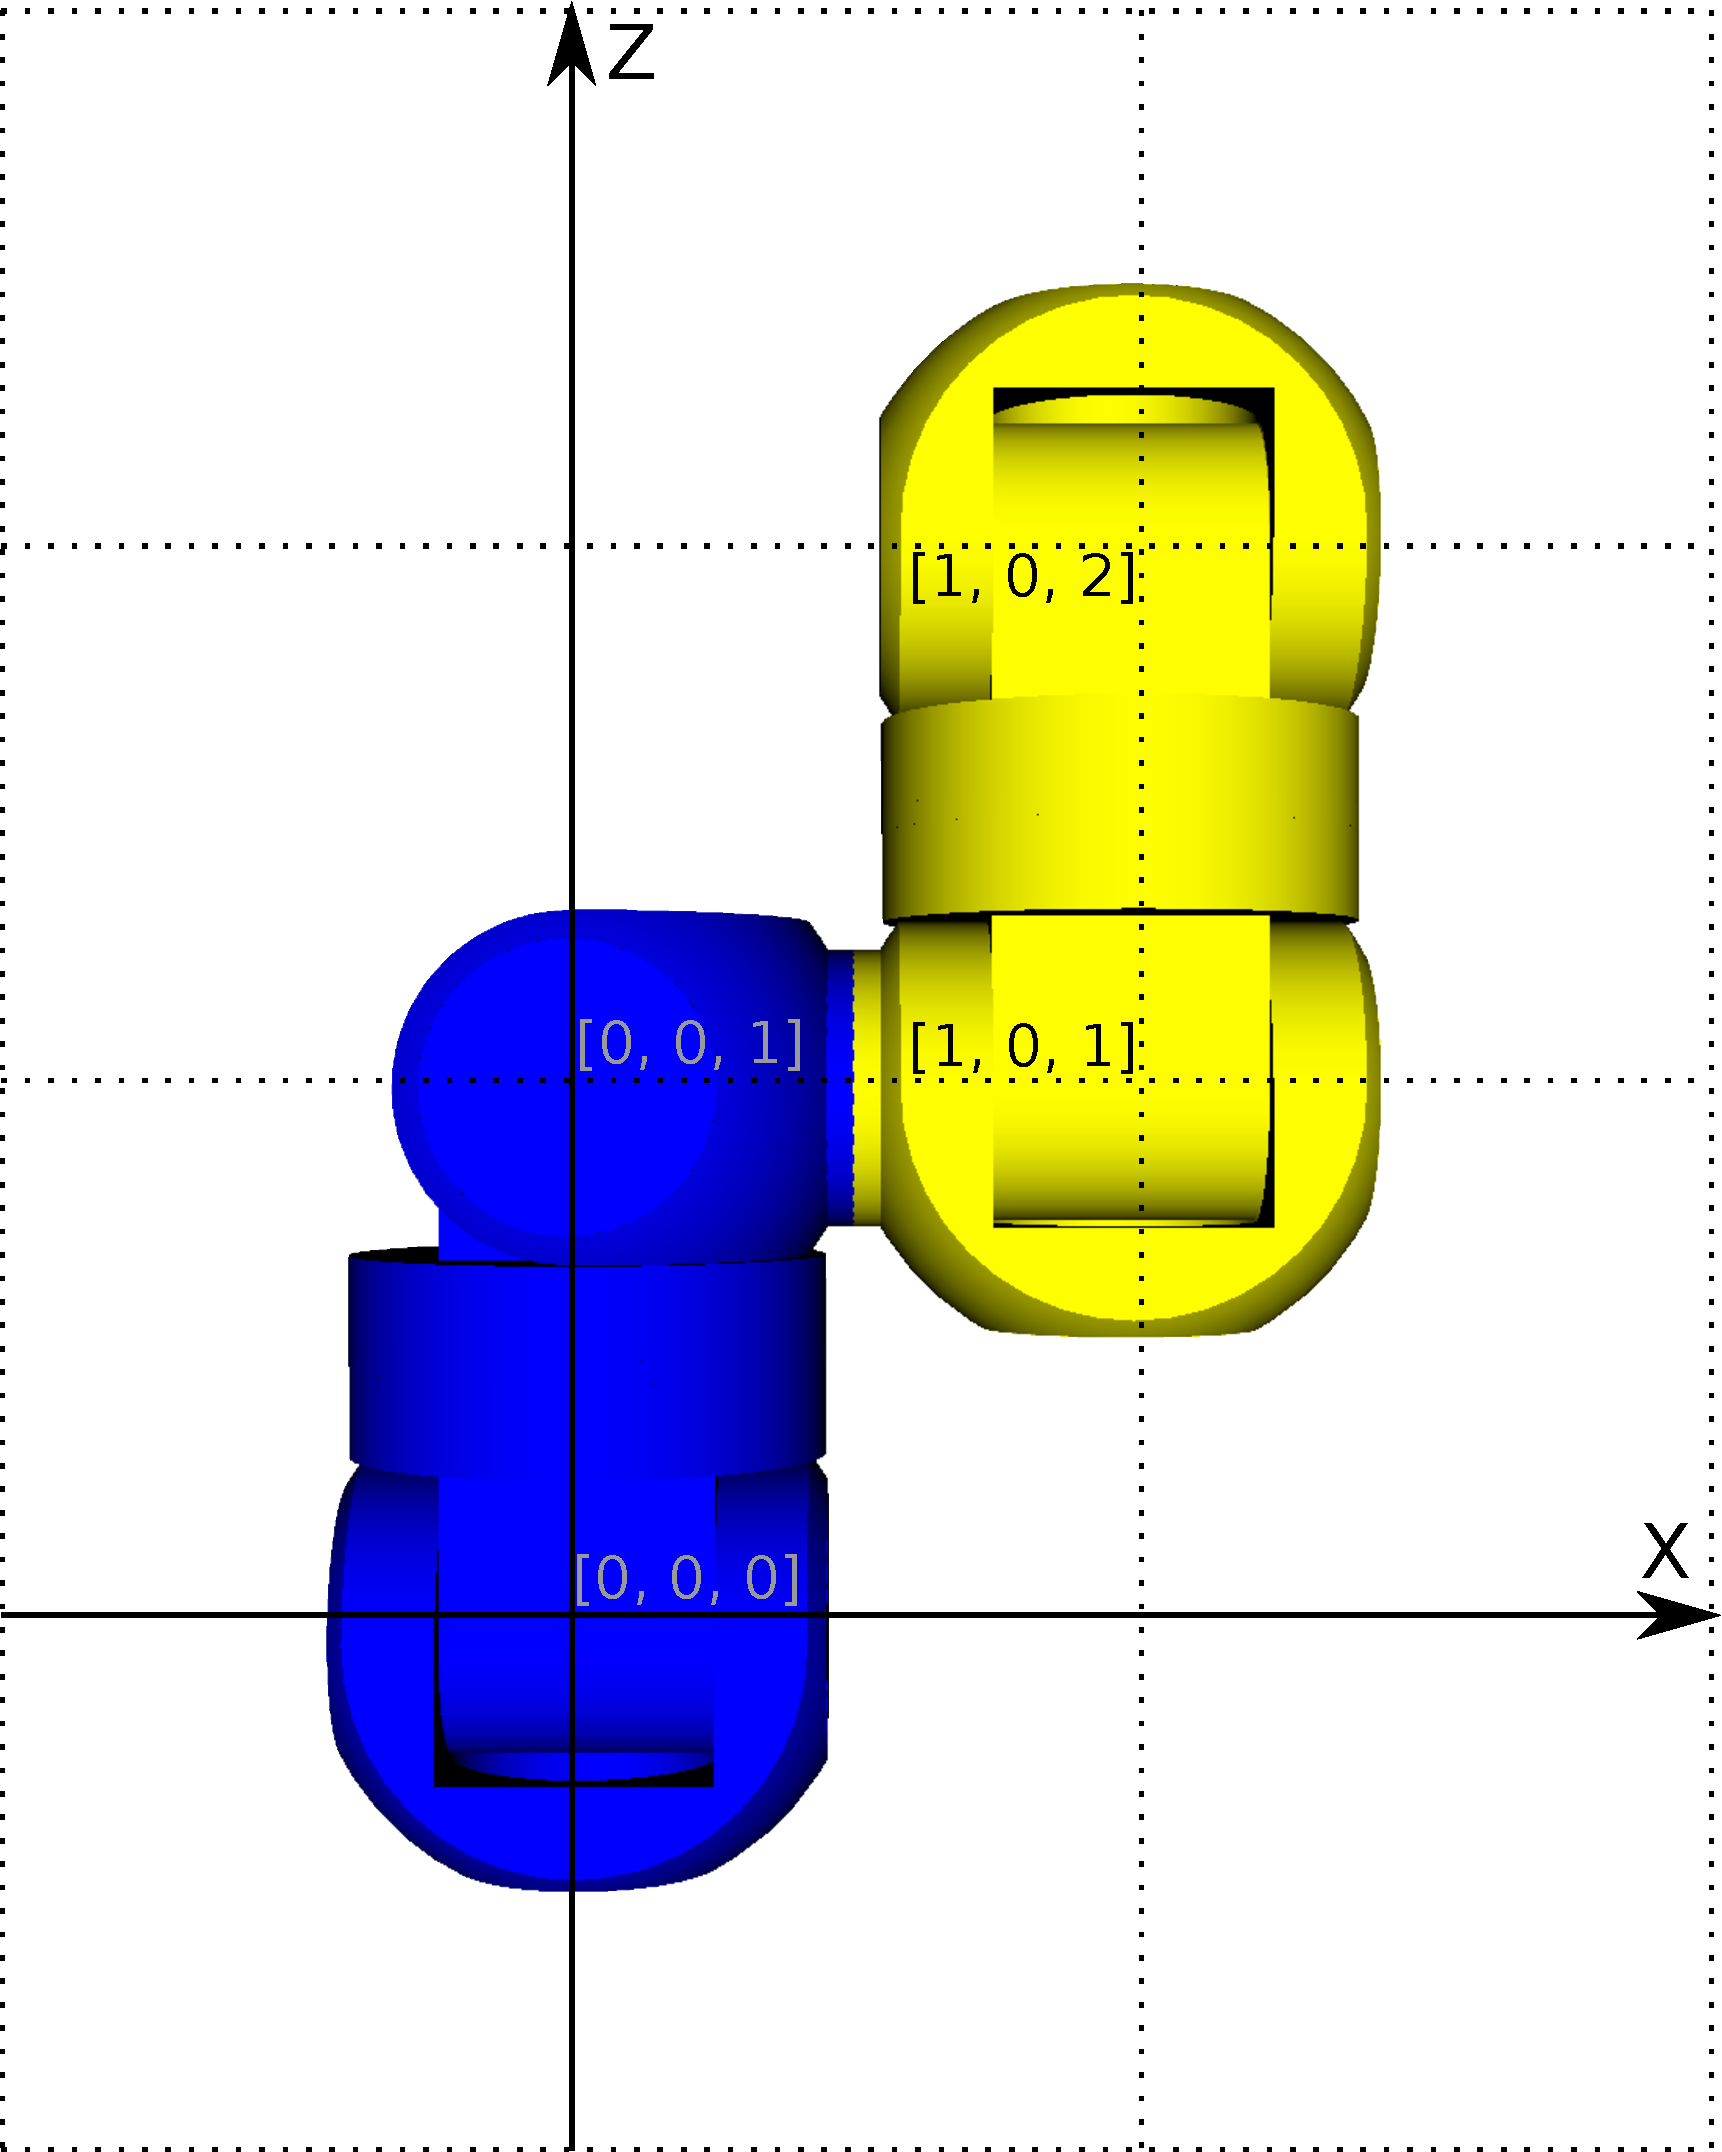
\includegraphics[width=0.5\textwidth]{pictures/module_coordinates.pdf}
    \caption[Ukážka súradnicového systému]{Príklad RoFIbota zasadeného do 3D súradnicového systému. Os $y$ smeruje od čitateľa. }
    \label{fig:moduleCoordinates}
\end{figure}

Algoritmus výpočtu súradníc v spomínanej diplomovej práci je založený na znalosti celej konfigurácie RoFIbota. V porovnaní s tým algoritmus na rekonfiguráciu popísaný v tejto kapitole znalosť celej konfigurácie RoFIbota nemá. Z tohto dôvodu je z algoritmu na výpočet súradníc použitá iba časť výpočtu matíc, z ktorých sa dajú súradnice modulu získať. Zvyšok bol pozmenený nasledovným spôsobom. 

Modul s najnižšou hodnotou \textit{id} pozná svoje súradnice (popísané vyššie). Následne každý modul, ktorý pozná svoje súradnice, vypočíta súradnice aj všetkým modulom, ktoré sú s ním spojený hranou. Tento výpočet dokáže vykonať každý modul, nakoľko pozná hodnoty svojich uhlov voľnosti, polohu konektorov a svoje vlastné súradnice. Následne pošle každému modulu, ktorý je s ním spojený hranou, správu o tom, aké súradnice má daný modul. Tento výpočet a rozposlanie správ sa dejú výhradne jednorázovo, nakoľko pri opakovaných výpočtoch a správach by došlo k cykleniu správ. Proces popísaný v tomto odseku sa opakuje, až kým nemá každý z modulov znalosť o svojich súradniciach. Algoritmus \ref{algorithm:coordinates} znázorňuje tento proces z pohľadu jedného modulu -- ide o program, ktorý má každý modul rovnaký. V tomto algoritme je v popise vstupu a výstupu stav algoritmu pred a po spustení. 

\begin{algorithm}
    \caption{Výpočet súradníc modulov RoFIbota. }
    \label{algorithm:coordinates}
    
    \DontPrintSemicolon
    \SetKwInOut{Input}{vstup}\SetKwInOut{Output}{výstup}
    \SetKwData{Id}{id}
    \Input{Konfigurácia RoFIbota bez znalosti zasadenia do~súradnicového systému.}
    \Output{Každý modul pozná svoje súradnice.}
    
    \If{\Id je najnižšie v RoFIbotovi}{
        inicializuj počiatočné súradnice\;
    }
    zdieľaj a príjmi informácie o znalosti súradníc\;
    \While{existuje modul, ktorý nepozná svoje súradnice}{
        \If{modul má známe súradnice {\bf and} tieto súradnice neboli zdieľané}{
            vypočítaj súradnice modulov, s ktorými mám hranu\;
            pošli im ich súradnice\;
        }
        zdieľaj a príjmi informácie o znalosti súradníc\;
    }
\end{algorithm}

Po tomto kroku má každý z modulov uložené, aká je jeho aktuálna pozícia v priestore, a teda môže prebiehať samotná rekonfigurácia. Základná myšlienka tejto rekonfigurácie je zachytená v algoritme \ref{algorithm:algo2}. 

Slovne, rekonfigurácia začína výberom modulu (označme ho ako $\mathcal{M}$) a akcie, ktorú sa pokúsi vykonať. Pred vykonaním samotnej akcie je nutné, aby pomocou komunikácie s ostatnými modulmi bolo zaručené, že danú akciu je možné bezpečne vykonať. Ak áno, tak sa vybraná akcia aj fyzicky vykoná, v opačnom prípade sa nevykoná žiadna zmena konfigurácie. Tento postup sa opakuje, až kým nenastane jedna z nasledujúcich podmienok: Prvá z nich je, že každý modul je v cieľovom stave, a druhá, že žiaden z modulov už nemôže vykonať žiadnu akciu. 

\begin{algorithm}
    \caption{Distribuovaná rekonfigurácia. }
    \label{algorithm:algo2}
    
    \DontPrintSemicolon
    \SetKwInOut{Input}{vstup}\SetKwInOut{Output}{výstup}
    \SetKwData{Modul}{$\mathcal{M}$}
    \SetKwData{Action}{action}
    \Input{Každý modul je v počiatočnom stave.}
    \Output{Každý modul je v cieľovom stave alebo žiaden z modulov už nedokáže vykonať žiadnu akciu.}
    
    \While{existuje modul, ktorý nie je v cieľovom stave \\ \hspace{35}{\bf and} existuje modul, ktorý môže vykonať nejakú akciu}{
        \Modul $\leftarrow$ vyber modul\;
        \Action $\leftarrow$ vyber prípustnú akciu pre \Modul\;
        \If{\Modul môže vykonať akciu \Action}{
            \Modul vykoná akciu \Action\;
        }
    }
\end{algorithm}

Ostáva teda popísať spôsob výberu modulu, akcie daného modulu, a to, akým spôsobom sa testuje, že je možné danú akciu bezpečne vykonať. 

Implementovaný algoritmus využíva na výber modulu hodnoty unikátnych identifikátorov modulov. Moduly sú zoradené podľa hodnoty \textit{id} od najnižšieho po najvyšší a algoritmus vyberá moduly v tomto poradí cyklicky. 

Akcie sa vyberajú tak, že sa preferujú rotácie pred prepojeniami. V prípade, že má modul každý stupeň voľnosti správne natočený, tak nasledujú odpojenia a vytváranie nových hrán sa deje ako posledné v poradí. Každá akcia je definovaná tak, že sa daný atribút zmení z aktuálneho stavu priamo do cieľového stavu. Pri vytváraní prepojení to je vytváranie prepojenia výhradne s modulmi, s ktorými je modul prepojený v cieľovom stave. Pri rotáciách ide o analógiu, teda rotácia z aktuálneho stavu uhla voľnosti do cieľového. Nakoľko žiaden modul nemá znalosť o celej konfigurácii RoFIbota, tak na testovanie validity akcie je nutné použiť výhradne vzájomnú komunikáciu medzi modulmi. 

Validita rotácie akéhokoľvek stupňa voľnosti je definovaná výhradne tým, že nedôjde k stretu žiadnych dvoch modulov. K stretu dvoch modulov dôjde iba v prípade, ak vzdialenosť stredov dotknutých strán modulov je menšia ako $1$. Je nutné otestovať, že počas celej rotácie nedôjde k stretu žiadnych dvoch modulov. 

Zadefinujme si množinu $\mathcal{R}$ ako množinu modulov, ktorej sa počas rotácie zmenia súradnice (budú premiestnené). Zvyšné moduly budú patriť do množiny, ktorú si označíme ako $\mathcal{S}$. Vykonávaním rotácie nesmie dôjsť ku kolízii, ale tú stačí definovať iba medzi modulmi z množiny $\mathcal{R}$ voči modulom z množiny $\mathcal{S}$. Kolízie medzi modulmi z množiny $\mathcal{S}$ nemôžu nastať, nakoľko sú všetky bez kolízií a ostávajú statické. V množine $\mathcal{R}$ sa súradnice modulov menia, ale ich vzájomná poloha ostáva nezmenená, a teda ku kolíziám nemôže dôjsť. 

Testovanie voči kolíziám prebieha nasledovne: $\mathcal{M}$ (vybraný modul) si zistí pozície modulov v množine $\mathcal{R}$ a na základe nich dokáže vypočítať, ako sa budú pohybovať stredy strán všetkých modulov v $\mathcal{R}$. Tieto pozície pošle $\mathcal{M}$ všetkým modulom v množine $\mathcal{S}$. Každý modul v $\mathcal{S}$ na základe vlastnej polohy v priestore dokáže určiť, či bude kolidovať s niektorým z modulov v množine $\mathcal{R}$ počas rotácie. Následne túto skutočnosť pošlú späť správou modulu $\mathcal{M}$. Z pozbieraných údajov o prípadných kolíziách dokáže $\mathcal{M}$ vyhodnotiť, či je rotácia bez kolízií. V prípade, že ku kolízii skutočne nedôjde, tak vykoná rotáciu a modulom z množiny $\mathcal{R}$ na záver rozpošle ich nové pozície v priestore. 

V porovnaní s rotáciou je validita prepojenie modulov definovaná iba na dvoch moduloch, ktoré prepojenie tvoria. Označme si preto modul, ktorý sa podieľa na prepojení ako druhý, ako $\mathcal{M}'$ a hranu, ktorá je vybraná na spojenie/odpojenie, ako $\mathcal{E}$. 

Validita akcie odpojenia dvoch modulov je definovaná výhradne spojitosťou RoFIbota po vykonaní akcie. Tá je definovaná tak, že existuje fyzická cesta medzi každými dvomi modulmi. 

\begin{lemma}
\label{lemma:disconnection}
RoFIbot zostane spojitý po odpojení hrany $\mathcal{E}$ práve vtedy, keď existuje cesta medzi modulmi $\mathcal{M}$ a $\mathcal{M}'$ taká, že neobsahuje túto hranu. 
\end{lemma}

\begin{proof}
Dôkaz lemmy \ref{lemma:disconnection} rozdelíme na dve časti. Prvá z nich je, že chceme dokázať, že ak existuje hrana s uvedenými podmienkami, tak RoFIbot ostane spojitý. Vezmeme si ľubovoľné dva moduly a chceme ukázať, že medzi nimi existuje fyzická cesta aj po odpojení. Cesty medzi týmito dvomi modulmi sa dajú rozdeliť podľa toho, či obsahujú alebo neobsahujú hranu $\mathcal{E}$: 
\begin{itemize}
    \item obsahuje -- cestu z pôvodnej konfigurácie je nutné pozmeniť, a to tak, že namiesto hrany $\mathcal{E}$ sa na toto miesto v ceste vloží iná cesta medzi modulmi $\mathcal{M}$ a $\mathcal{M}'$, 
    \item neobsahuje -- cestu z pôvodnej konfigurácie nie je nutné meniť, nakoľko všetky hrany budú naďalej existovať.
\end{itemize}

Ostáva ukázať, že ak je RoFIbot spojitý aj po rozpojení, tak v pôvodnej konfigurácii existovala cesta z $\mathcal{M}$ do $\mathcal{M}'$ neobsahujúca hranu $\mathcal{E}$. Keďže je konfigurácia po zmene spojitá, tak z definície musí existovať cesta z $\mathcal{M}$ do $\mathcal{M}'$ a zároveň neobsahuje hranu $\mathcal{E}$, lebo táto hrana sa v zmenenej konfigurácii už nenachádza. Zároveň vieme, že sa konfigurácia inak nezmenila, takže táto cesta musí existovať aj v pôvodnej konfigurácii, čím sme dokázali lemmu. 

\end{proof}

Z toho vyplýva, že stačí zistiť, či existuje cesta popísaná v lemme~\ref{lemma:disconnection}. Modulu $\mathcal{M}$ pošlú všetky moduly informáciu, s akými ostatnými modulmi sú prepojené. Z týchto údajov si modul $\mathcal{M}$ dokáže vytvoriť neorientovaný súvislý graf, kde každý modul je vrcholom a prepojenie medzi modulmi je hranou v grafe. Zároveň je v grafe povolené mať aj viacnásobné hrany medzi vrcholmi (maximálne však môžu existovať dve hrany medzi rovnakými vrcholmi). Hranu $\mathcal{E}$ do tohto grafu nepridávame (je to graf reprezentujúci konfiguráciu po odpojení). Následne pomocou \textit{BFS} z vrcholu ekvivalentnému modulu $\mathcal{M}$ vyhľadáme cestu do vrcholu ekvivalentnému modulu $\mathcal{M}'$. Keďže tento výpočet prebieha nad konečným grafom, tak zaručene skončí. Odpojenie môžeme vykonať iba v prípade, ak prehľadávanie do šírky nájde cestu do požadovaného vrcholu. 

Posledným typom akcie, ktorú môže vybraný modul vykonať, je pripojenie k inému modulu. V tomto prípade je pre validitu tejto akcie postačujúce, ak druhý modul spojenia (označme ho opäť ako $\mathcal{M}'$) je schopný zadaného prepojenia. Inak povedané, nachádza sa na správnych súradniciach a zároveň je správne natočený (správnym konektorom a jeho natočením voči konektoru modulu $\mathcal{M}$). Tieto súradnice a natočenia dokáže určiť modul $\mathcal{M}$ zo svojej polohy v priestore a z hodnôt uhlov voľnosti. Stačí teda, aby prebehla komunikácia medzi $\mathcal{M}$ a $\mathcal{M}'$, či $\mathcal{M}'$ má požadovanú polohu v priestore a správne natočenie. V prípade, že je všetko podľa požiadaviek na spojenie, prebehne spojenie modulov. 

% ------------------------------------------------------ 2 ------------------------------------------------------



% ------------------------------------------------------ 3 ------------------------------------------------------

\chapter{Implementácia}
\label{sec:implementation}
Platforma RoFI je open-source projekt. Implementačná časť tejto práce je súčasťou knižnice RoFILib\footnote{\url{https://github.com/paradise-fi/RoFI/tree/master/RoFILib}}, ktorá sa zaoberá vývojom simulácií a vizualizácie. 

RoFILib je knižnica naprogramovaná v jazyku C++. Táto knižnica poskytuje funkcie na simuláciu rekonfigurácie rôznymi algoritmami a z rôznych pohľadov (centralizovaný a distribuovaný) na problém rekonfigurácie. V súčasnej dobe sú to algoritmy navrhnuté v rámci tejto práce a v diplomovej práci \textit{Motion Planning for the RoFI Platform} \cite{vozarovaMasterThesis}.

Knižnica zároveň poskytuje možnosť vizualizácie konfigurácií a rekonfigurácií RoFIbotov. Vizualizér vznikol ako bakalárska práca \textit{Vizualizace pro robotickou platformu RoFI} \cite{nausovaBachelorThesis} a dokáže produkovať obrázky konfigurácie alebo videá rekonfigurácie. Väčšina obrázkov, ktoré sú súčasťou tejto práce a jej príloh, sú výstupom vizualizéru. 

\section{Technická špecifikácia a využité knižnice}
\label{sec:libraries}
Problémy rekonfigurácie, ktoré riešia spomínané práce, majú jednotné vstupy a výstupy: Na vstupe sa nachádzajú dva súbory, ktoré popisujú počiatočnú a cieľovú konfiguráciu RoFIbota, ktorý sa má rekonfigurovať. Výstupom je súbor, ktorý obsahuje zoznam konfigurácií RoFIbota, ktoré vznikli po každom kroku rekonfigurácie. 

Podrobný popis vstupných a výstupných súborov sa nachádza v diplomovej práci \textit{Motion Planning for the RoFI Platform} \cite{vozarovaMasterThesis}. Keďže definícia vstupov a výstupov pre rekonfiguračné problémy je jednotná, tak je zaručená kompatibilita aj s vizualizačným programom knižnice RoFILib. 

Vstupné a výstupné súbory obsahujú celú konfiguráciu RoFIbota, ktorej celková znalosť na vstupe simulácie ľubovoľného modulu nie je pre túto prácu možná. Tým pádom je z dôvodu kompatibility so zvyškom knižnice implementovaný aj preprocessing a postprocessing, ktorý obaľuje tu implementované algoritmy. 

Táto práca je zameraná na distribuované algoritmy a tie sú navrhnuté tak, aby každý modul RoFIbota fungoval ako samostatná entita. Komunikácia medzi entitami je možná výhradne pomocou správ, ktorá je vo fyzických modulov uskutočnená pomocou protokolu MPI\footnote{Message Passing Interface}. 

Z týchto dôvodov je implementácia navrhnutých algoritmov napísaná v jazyku C++ s využitím knižnice OpenMPI \cite{openMPILibrary}. 

OpenMPI je open-source knižnica \cite{openMPIGit}, ktorá uľahčuje vývoj multiprocesových aplikácií v distribuovanom prostredí. Keďže je táto knižnica viacúčelová, tak sú v tejto práci využité napríklad aj nasledujúce súčasti: Spustenie zadaného počtu procesov s rovnakým programom s unikátnou identifikáciou (tzv. \textit{rank} procesu). Komunikácia medzi zadanými procesmi (napríklad posielanie správ medzi dvomi konkrétnymi procesmi, broadcast alebo all-to-all komunikácia). 

Simulácia prebieha tak, že každý modul je samostatný proces, ktorý dostane na vstup vstupné informácie (svoj počiatočný a cieľový stav). Spustené procesy si následne medzi sebou vymieňajú správy na základe tejto komunikácie prebiehajú výpočty a validné akcie tak, aby sa každý modul rekonfiguroval z počiatočného stavu do cieľového stavu. 

Aby bol výstup tejto práce plne kompatibilný s vizualizérom knižnice RoFILib, tak sú jednotlivé vykonané akcie zapísané do logu. Na tie sa po skončení rekonfigurácie spustí postprocessing, ktorý vytvorí výstup kompatibilný so zvyškom knižnice. 

Keďže ide o simuláciu, tak jej cieľom je priblížiť sa čo najviac fyzickému modelu rekonfigurácie RoFIbota. To znamená, že algoritmy využívajú iba minimálnu sadu funkcií a možností knižnice OpenMPI, a to tie, ktoré je možné využiť vo fyzických moduloch. Príkladom tohto obmedzenia je nevyužívanie zdieľanej pamäte, nakoľko fyzické moduly žiadnu zdieľanú pamäť nemajú. 

Na praktické využitie knižnice na simuláciu rekonfigurácie a vizualizácie je nutné mať nainštalované nasledujúce knižnice: 
\begin{itemize}
    \item C++ kompilátor, ktorý podporuje štandard aspoň C++17, 
    \item \texttt{cmake} verzie aspoň 3.10 -- v prípade prekladu na základe súborov CMakeLists, 
    \item knižnica \texttt{Armadillo} -- slúži na prácu s maticami a vektormi, ktoré sú potrebné na výpočty rekonfigurácie,  
    \item knižnice \texttt{VTK}, \texttt{FFmpeg} a grafický editor \texttt{Inkscape} -- pre správne fungovanie vizualizačného nástroja, 
    \item knižnica \texttt{openMPI} -- na kompiláciu a spustenie distribuovaných algoritmov. 
\end{itemize}

 Návody na ich inštaláciu sa nachádzajú v súbore \texttt{README.md}\footnote{\url{https://github.com/paradise-fi/RoFI/blob/master/RoFILib/README.md}} knižnice RoFILib. 

Knižnica openMPI spúšťa procesy tak, aby každý z nich mal k dispozícii samostatné jadro, a to hlavne z dôvodu, aby sa navzájom neovplyvňovali\footnote{\url{https://www.open-mpi.org/faq/?category=running#oversubscribing}}. Preto je nutné, aby hardvérové vybavenie strojov, na ktorých bude bežať rekonfigurácia mala aspoň toľko jadier procesoru ako je počet modulov RoFIbota. 

\newcommand{\comment}[1]{}
\comment{
Z pohľadu hardvérového vybavenia sú kladené obmedzenia výhradne pri používaní distribuovanej rekonfigurácie. Nakoľko je každý modul reprezentovaný jedným procesom, tak je nutné mať hardvér, ktorý je schopný pustiť toľko procesov ako je počet modulov RoFIbota, ktorého rekonfiguráciu ideme simulovať. }

\section{Použitie}
Samotné spustenie algoritmov na rekonfiguráciu popísaných v tejto práci je možné buď ručným spustením, alebo využitím pripraveného skriptu. V prípade nevyužitia skriptu je nutné, aby vstup pre samotný algoritmus rekonfigurácie bol v špecifickom tvare. Ten je zhodný so súbormi, ktoré vytvára preprocessing. 

Preprocessing slúži na to, aby z konfiguračných súborov kompatibilných s knižnicou RoFILib vytvoril súbory pre distribuovanú rekonfiguráciu. Na jeho výpočet je nutné zadať mu súbory s počiatočnou a cieľovou konfiguráciou RoFIbota a adresár, kde môže vytvárať pomocné súbory. Medzi nepovinné parametre patria názvy súborov pre počet modulov a slovník. 

Výsledkom preprocessingu je príprava všetkých potrebných súborov na to, aby bolo možné využiť program na rekonfiguráciu a následný postprocessing. Toto sú všetky potrebné: 
\begin{itemize}
    \item súbory \texttt{id.init} a \texttt{id.goal} (pre všetky \textit{id} modulov RoFIbota) -- obsahujú počiatočný resp. cieľový stav modulu s identifikátorom \textit{id}, 
    \item súbory \texttt{count} -- obsahuje počet modulov v konfigurácii, resp. hodnotu $-1$ ak nastal prípad, že počet modulov v počiatočnej a cieľovej konfigurácii nie je zhodný (teda rekonfigurácia nie je možná), 
    \item súbory \texttt{dictionary} -- obsahuje slovník medzi pôvodnými identifikátormi modulov a identifikátormi využívanými pre rekonfiguráciu
\end{itemize}

Dôvod zavedenia súboru \texttt{count} je, že tento súbor slúži na to, aby bolo možné rýchlo zistiť koľko procesov je nutné spustiť na rekonfiguráciu. Zavedenia slovníka je potrebné, nakoľko algoritmy navrhnuté v tejto práci predpokladajú, že moduly majú hodnoty \textit{id} z množiny $\interval[0, n - 1)$, kde $n$ je počet modulov RoFIbota.

Príklad spustenia preprocessingu, kde \mintinline{text}{init} a \mintinline{text}{goal} sú súbory obsahujúce počiatočnú a cieľovú konfiguráciu RoFIbota a \mintinline{text}{dir} je adresár, kde sa budú ukladať pomocné súbory:

\begin{minted}{bash}
./rofi-distribute-preprocessing -i init -g goal -d dir
\end{minted}.

%%%%%%%%%%%%%%%%%%%%%%%%%%%%%%%%%%%%%%%%%%%%%%%%%%%%%%%
% tie prepinace treba prejst kvoli readme.. 

\comment{
Plný výpočet prepínačov preprocessingu, pričom platí, že prepínače na súbory počiatočnej a cieľovej konfigurácie RoFIbota sú povinné: 
\begin{minted}{text}
  -h, --help            Print help
  -i, --init arg       Initial config file
  -g, --goal arg        Goal config file
  -d, --directory arg   Directory for module's configs
  -c, --count arg       File name for module's count file
  -t, --dictionary arg  File name for module's dictionary
\end{minted}}
%%%%%%%%%%%%%%%%%%%%%%%%%%%%%%%%%%%%%%%%%%%%%%%%%%%%%%%%
Ak sú vstupné súbory pripravené v tvare, ktorý vyžadujú algoritmy na rekonfiguráciu, tak je možné spustiť samotnú rekonfiguráciu. Samotný program vyžaduje adresár, v ktorom sa nachádzajú vyššie popísané súbory s počiatočným a cieľovým stavom každého modulu v samostatnom súbore. Okrem toho vyžaduje aj algoritmus, ktorý má použiť na výpočet rekonfigurácie. 

\comment{Prehľad algoritmov je nasledovný: 

\begin{minted}{text}
  full     Full configuration knowledge
  partial  Patrial configuration knowledge 
           - full distributed
\end{minted}}

V prípade výberu algoritmu s plnou znalosťou konfigurácie je možné zvoliť aj heuristiku pre výpočet algoritmu \textit{A*}. Podrobný popis princípov heuristík je popísaný v diplomovej práci \textit{Motion Planning for the RoFI Platform} \cite{vozarovaMasterThesis}. \comment{Ich kompletný výpočet je: 

\begin{minted}{text}
  trivial  All configurations have value 1 (default)
  dMatrix  Module matrices difference
  dCenter  Module center difference
  dJoint   Joint difference
  dAction  Action difference
\end{minted}

Samotný program na rekonfiguráciu má definované nasledujúce prepínače: 

\begin{minted}{text}
  -h, --help           Print help
  -d, --directory arg  Directory for module's configs
  -a, --alg arg        Algorithm for reconfiguration: 
                       full, partial
  -e, --eval arg       Evaluation function for full 
                       algorithm for A*: trivial, 
                       dMatrix, dCenter, dJoint, dAction
\end{minted}}

Výpočet algoritmu na rekonfiguráciu však prebieha tak, že sa spustí viacero procesov naraz. Toto umožňuje knižnica OpenMPI a to pomocou príkazu \mintinline{bash}{mpiexec} s vhodnými prepínačmi. Je nutné nastaviť počet procesov pomocou prepínača \mintinline{bash}{-np}. Zároveň je možné spúšťať tieto procesy plne distribuovane, teda na viacerých strojoch naraz, a tie sa špecifikujú prepínačom \mintinline{bash}{--hostfile} \cite{openMPIHostFile} s názvom súboru, ktorý obsahuje zoznam hostiteľských strojov. 

Nech \mintinline{text}{host-file} je súbor so špecifikovanými hostiteľskými strojmi a \mintinline{text}{dir} je adresár, v ktorom sú súbory s počiatočnými a cieľovými stavmi modulov. Príkaz na spustenie napríklad algoritmu s plnou znalosťou konfigurácie RoFIbota na rekonfiguráciu $4$ modulov s triviálnou heuristikou je: 
\begin{minted}{bash}
mpiexec --hostfile host-file -np 4 
  ./distribute/rofi-distribute -d dir -a full -e trivial
\end{minted}.

Výstup algoritmu je vypísaný na štandardný výstup. Jeho formát je nasledovný: Na úplnom začiatku je uvedená počiatočná konfigurácia RoFIbota tak, že každý riadok konfigurácie obsahuje prefix $0$. Nakoľko program nemá plnú znalosť konfigurácie, tak ju vytvorí tak, že každý modul vypíše svoj stav. Nasledujúce riadky obsahujú vykonané akcie, pričom ich poradie nemusí byť zhodné s poradím, v akom sa dané akcie vykonávali. Preto má každá akcia na začiatku svojho zápisu kladný celočíselný prefix, ktorý hovorí o poradovom čísle kroku, v ktorom sa daná akcia vykonala. Zároveň sa predpokladá, že výstup obsahuje všetky poradové čísla krokov (teda v každom kroku sa vykoná vždy aspoň jedna akcia). Ak je použitý druhý algoritmus a nastane prípad, že rekonfigurácia už nemôže pokračovať, ale aspoň jeden modul nie je v cieľovej konfigurácii, tak na konci výstupu je poznámka o skutočnosti, že sa nejedná o cieľový stav RoFIbota. 

Tento výstup však nie je kompatibilný so zvyšnými časťami knižnice RoFILib. Na to, aby bola zaručená kompatibilita, tak je možné využiť časť postprocessing. 

Cieľom postprocessingu je vytvoriť súbor, ktorý obsahuje postupnosť konfigurácií rekonfigurácie RoFIbota, pričom na vstupe má súbor, kde sú časovými známkami označené počiatočná konfigurácia a akcie, ktoré sa na danej konfigurácii majú vykonáva. Teda postprocessing vezme súbor s akciami a postupne ich podľa časových známok aplikuje na počiatočnú konfiguráciu. Zároveň aj premenuje identifikátory modulov podľa zadaného slovníka, ktorý bol napríklad vytvorený ako produkt preprocessingu. 

Nech \mintinline{text}{file} je súbor, ktorý obsahuje hodnoty, ktoré sú zhodné s popisom výstupu rekonfiguračného algoritmu a \mintinline{text}{dictionary} je súbor, v ktorom je uvedený slovník zmien unikátnych identifikátorov modulov, tak postprocessing môže byť spustený napríklad takýmto príkazom: 
\begin{minted}{bash}
./rofi-distribute-postprocessing -i file -t dictionary
\end{minted}

\comment{
Oba vyššie uvedené prepínače sú povinné. Prehľad všetkých prepínačov pre postprocessing je nasledujúci: 

\begin{minted}{text}
  -h, --help            Print help
  -t, --dictionary arg  Dictionary file
  -i, --input arg       File with time marked actions 
\end{minted}}

Toto je kompletné využitie časti \textit{distribute} knižnice RoFILib, ktorá vznikla ako implementačná časť tento bakalárskej práce. Nakoľko je z dôvodu kompatibility s knižnicou nutné spúšťať preprocessing a postprocessing, tak je pripravený aj skript, ktorý túto sekvenciu spúšťania všetky časti automaticky. 

Zoznam a podrobný popis všetkých prepínačov, ktoré sa využívajú v jednotlivých častiach a skripte sa nachádzajú v \texttt{README.md}\footnote{\url{https://github.com/paradise-fi/RoFI/blob/master/RoFILib/README.md}}. 

\comment{
Pripravený skript má nasledujúcu sadu prepínačov: 
\begin{minted}{text}
  -h, --help           Print help
  -i, --init arg       Initial config file
  -g, --goal arg       Goal config file
  -d, --directory arg  Directory for module's configs
  -f, --hostfile arg   Host file for mpiexec
  -a, --alg arg        Algorithm for reconfiguration: 
                       full, partial
  -e, --eval arg       Evaluation function for full 
                       algorithm for A*: trivial, 
                       dMatrix, dCenter, dJoint, dAction
  -c, --noclear        Do not clear temporary files
  -o, --output arg     Output file name
\end{minted}

Prepínače \mintinline{text}{-i}, \mintinline{text}{-g} a \mintinline{text}{-d} sú zhodné s prepínačmi v preprocessingu a prepínače \mintinline{text}{-a} a \mintinline{text}{-e} ako v spúšťaní rekonfigurácie. Prepínačom \mintinline{text}{-f} sa nastavuje \textit{hostfile} pre spúšťanie rekonfigurácie pomocou \mintinline{bash}{mpiexec}. }






% ------------------------------------------------------ 3 ------------------------------------------------------




% ------------------------------------------------------ 4 ------------------------------------------------------
\chapter{Experimentálne vyhodnotenie}
Oba navrhnuté a implementované algoritmy boli otestované na vzorových vstupoch. Vyhodnotenie spočíva v porovnávaní časov, ktorý bol nutný na ich výpočet, schopnosti nájsť riešenie a zároveň aj porovnávanie dĺžok nájdených rekonfiguračných postupností. 

\section{Ukážkové rekonfigurácie}
Vzorové vstupy vznikli generátorom konfigurácií\footnote{\url{https://github.com/paradise-fi/RoFI/tree/master/RoFILib/generate}}, ktorý patrí do knižnice RoFILib. 

Testované vstupy sú vybrané tak, že ich počiatočná konfigurácia je vygenerovaná náhodne s tým, že má predom určený počet modulov. Tie sú vybrané tak, aby pokryli rôzne veľkosť RoFIbotov od malých konfigurácií s $2$, $3$ alebo $5$ modulmi po veľké konfigurácie s $15$, $50$ a $80$ modulmi. Vybrané počiatočné konfigurácie sú zobrazené na obrázku~\ref{fig:rofibotExamples}. 

Cieľová konfigurácia je vygenerovaná tak, že generátor vygeneruje zadaný počet validných krokov, ktoré sa majú vykonať na počiatočnej konfigurácií a tie sa aplikujú na túto konfiguráciu. Tento prístup zaručuje, že existuje rekonfiguračná postupnosť a dokonca jej dĺžku dokážeme zadanou hodnotou zhora ohraničiť. Vzorové vstupy sú generované na rekonfigurácie dĺžok $5$, $10$, $20$, $30$ a $50$ krokov. 

Každý vstup má na základe týchto údajov aj určené značenie. Názvy vstupných súborov majú nasledujúci formát \textit{<počet modulov>-<počet krokov>-\{init, goal\}.in}, teda napríklad súbor s popisom konfigurácie na obrázku \ref{fig:3-10-init} sa nazýva \textit{3-10-init.in}, nakoľko ide o konfiguráciu s $3$ modulmi, ktorá bola generovaná na rekofiguráciu o $10$ krokoch. 

\begin{figure}[hbt!]
    \centering
    \begin{subfigure}[b]{0.47\textwidth}
        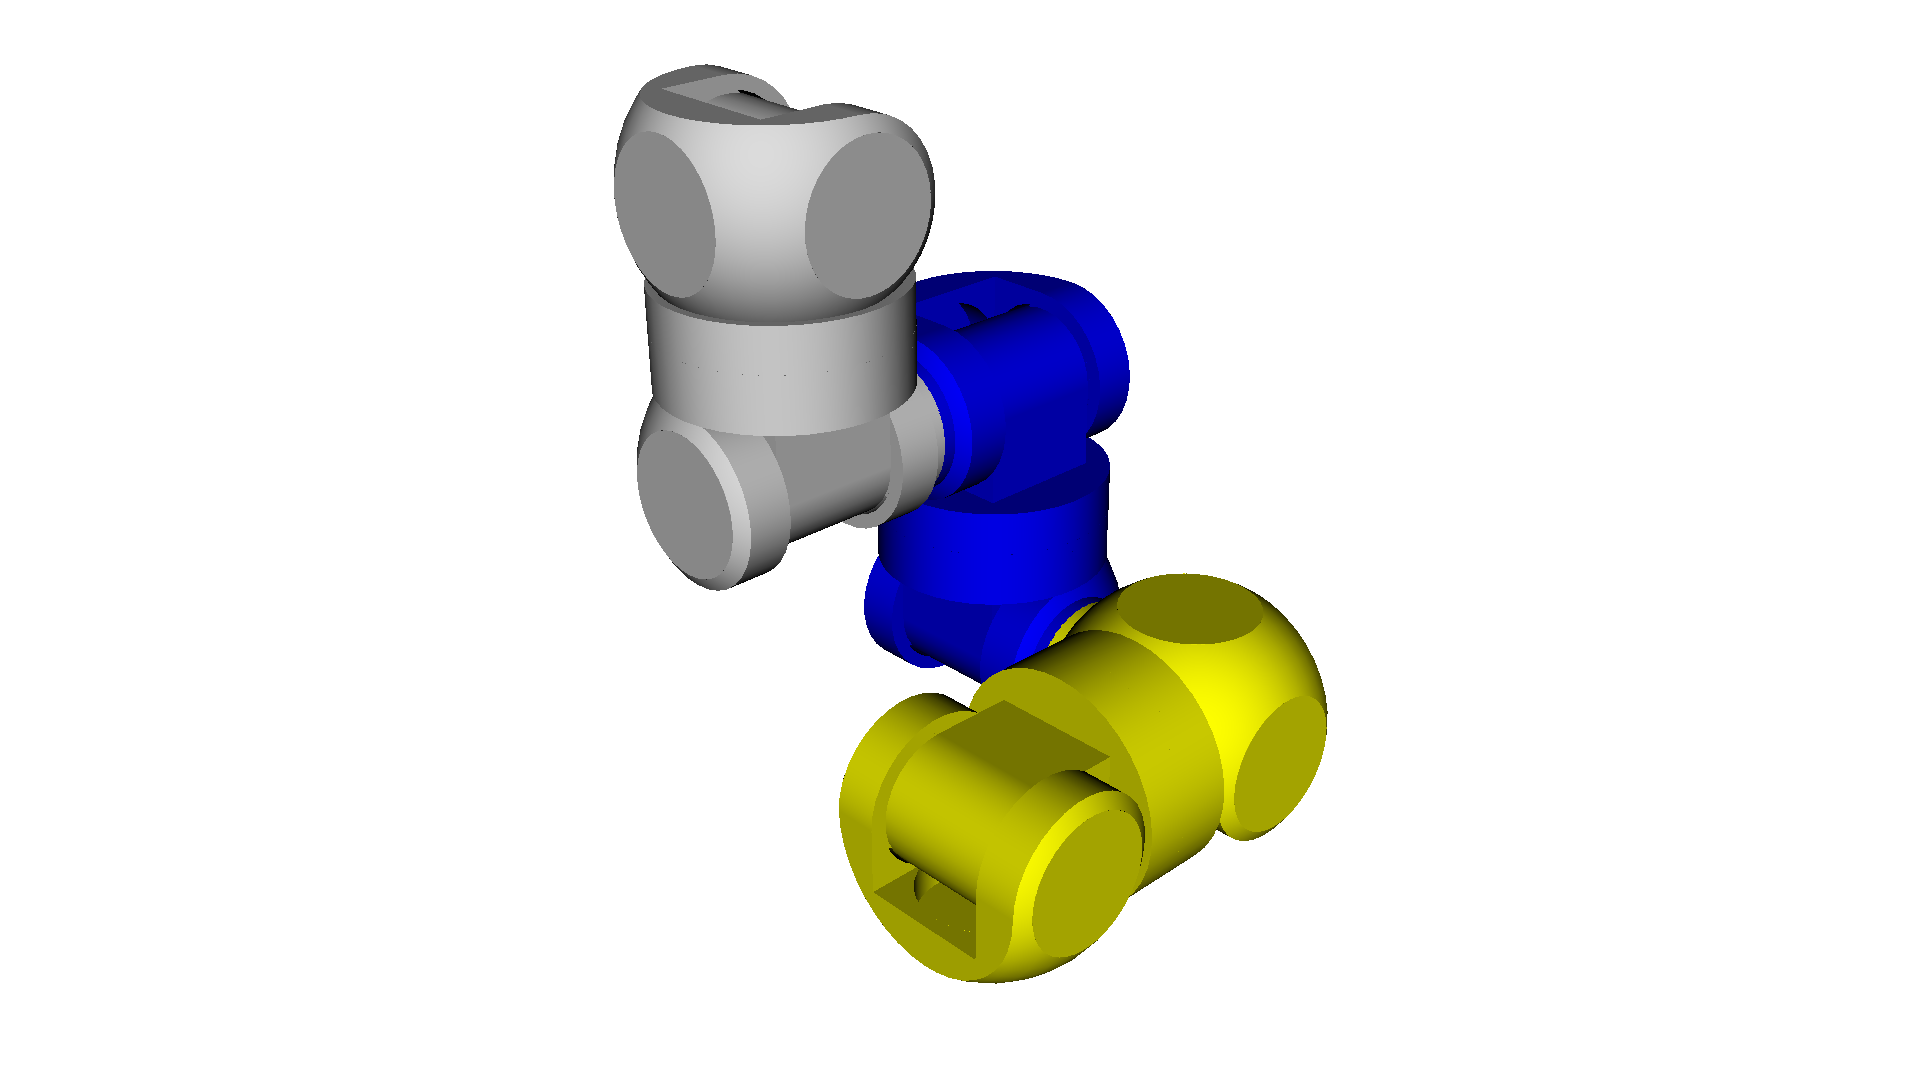
\includegraphics[width=\textwidth]{pictures/3-10-init.png}
        \caption[3-10-init]{Vstupná konfigurácia $3$-$10$.}
        \label{fig:3-10-init}
    \end{subfigure}
    \begin{subfigure}[b]{0.47\textwidth}
        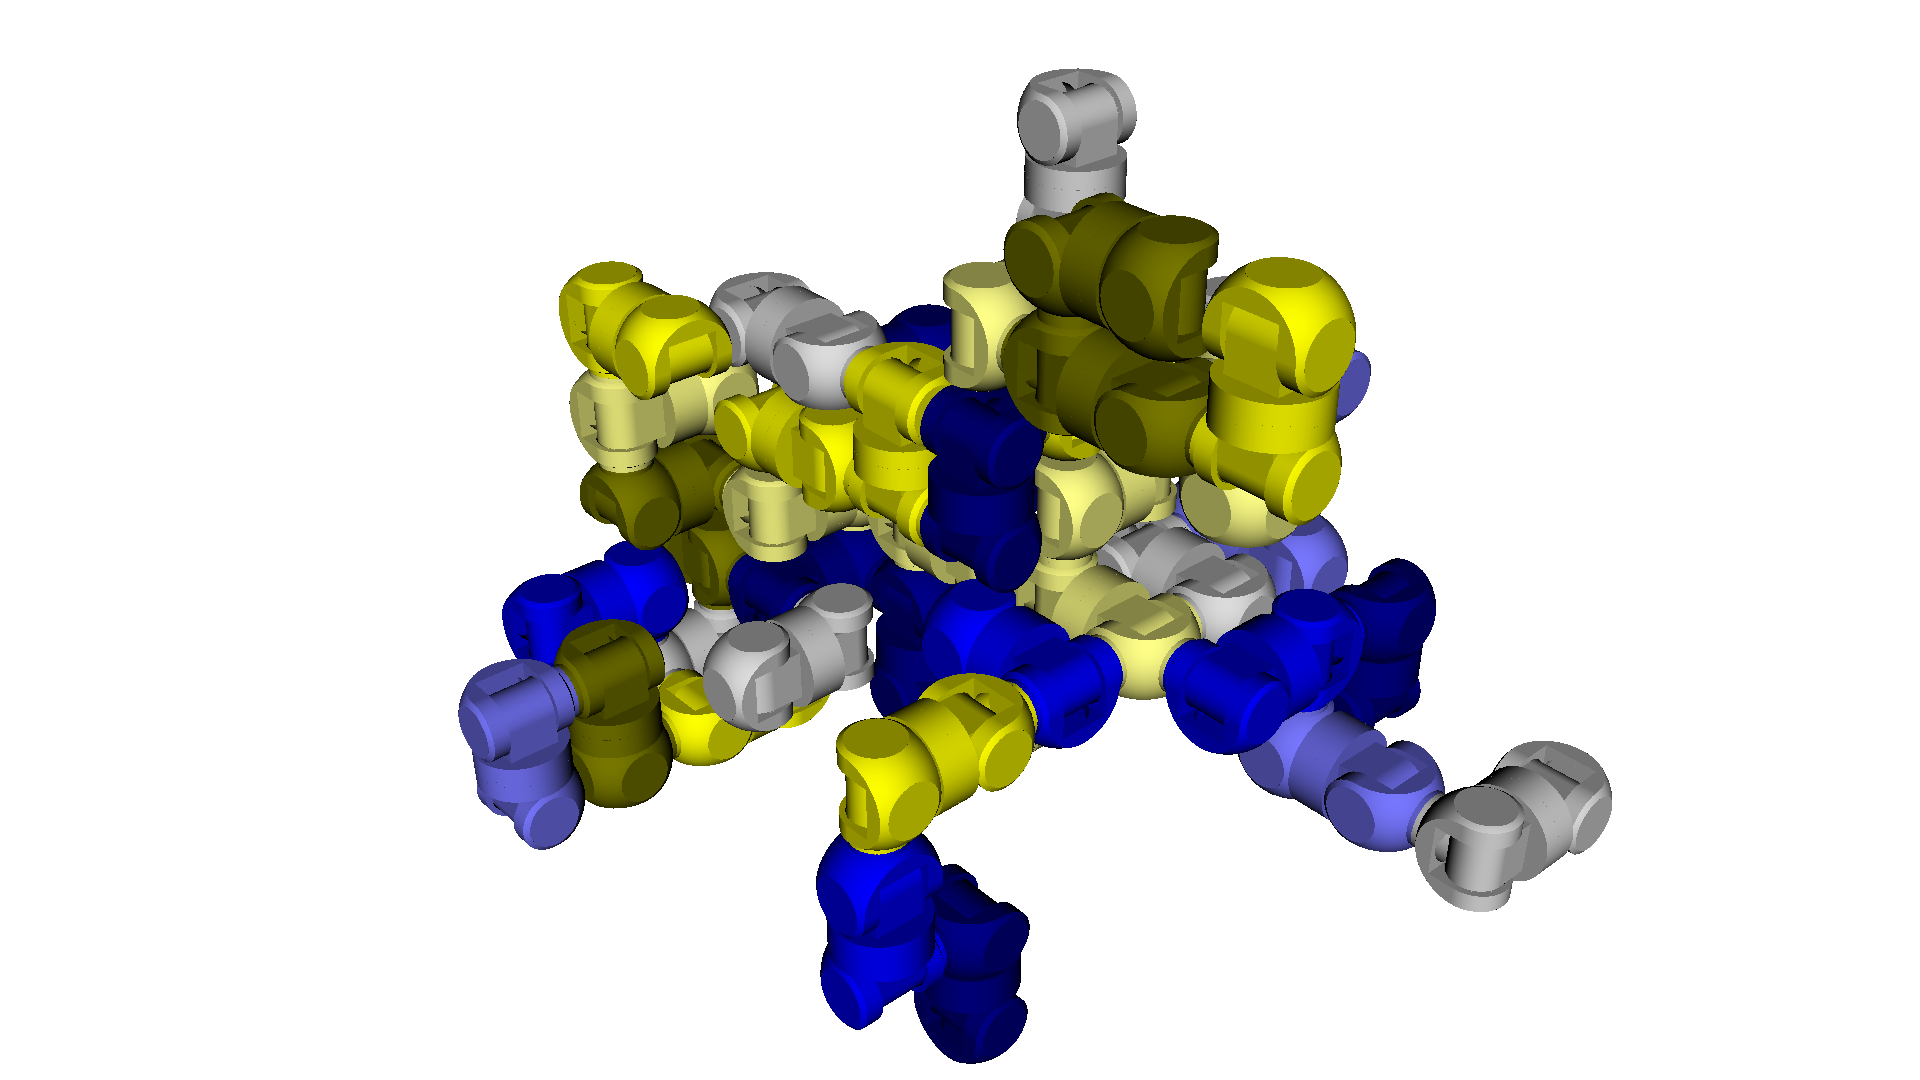
\includegraphics[width=\textwidth]{pictures/50-5-init.png}
        \caption[50-5-init]{Vstupná konfigurácia $50$-$5$.}
    \end{subfigure}
    \caption[Ukážkové vstupné konfigurácie]{Ukážka vstupných konfigurácií vygenerovaných náhodne. }
    \label{fig:rofibotExamples}
\end{figure}

Okrem náhodne generovaných vstupov boli skúšané aj ručne vytvorené vstupy, kde nie je nutne zaručená existencia cesty rekonfigurácie. Niektoré príklady vizualizuje obrázok \ref{fig:rotationExampleByHand}. 

Nakoľko algoritmy navrhnuté v tejto práci potrebujú dostatočný počet jadier procesorov, tak boli vstupy spúšťané na príslušnom počte strojov z $20$ hardvérovo zhodne vybavených strojov. Každý z nich má štvorjadrový procesor \texttt{Intel Xeon 5130} o takte $2.00$\,GHz a $16$\,GB RAM. 

\section{Evaluácia výsledkov na vzorových príkladoch}
-- Porovnanie algoritmov z pohľadu časovej a priestorovej zložitosti

-- Popis, ktorý algoritmus a na aké konfigurácie a zmeny v rekonfiguráciách je viac vhodný


--------------------------------------


-- Ukážkové konfigurácie a porovnanie rýchlostí ich výpočtov a prípadne rôznorodosti nájdených riešení

-- Odkazy na videá, obrázky, presné časy behov a rôznosť riešení. 

% ------------------------------------------------------ 4 ------------------------------------------------------





% ------------------------------------------------------ 5 ------------------------------------------------------
\chapter{Záver}
\label{sec:future}
// Rekapitulácia. 

// Ako ďalej zlepšovať algoritmy a čo ešte pridávať a podobne. 

Navrhnuté algoritmy nehľadajú optimálne riešenie a to hlavne z dôvodu časovej zložitosti výpočtov. Algoritmy sú, ale navrhnuté tak, aby sa dali jednoducho modifikovať a optimalizovať. V prípade prvého algoritmu ide hlavne o samotný výpočet postupnosti krokov rekonfigurácie a jej optimalizáciu. 

V súčasnej dobe je tento algoritmus implementovaný tak, že každý modul počíta rovnaké hodnoty a na základe nich sa následne vykonáva fyzická rekonfigurácia. Jedným z návrhov na zlepšenie tohto algoritmu je, že každý z modulov môže počítať postupnosť krokov rôznymi algoritmami a inými heuristikami. Okrem toho je prístup optimalizácie krokov greedy, a teda nemusí vždy nájsť optimálne riešenie. Teda ďalším zlepšením je riešenie optimalizácie iným spôsobom a vzájomnou komunikáciou sa dohodnú, či je lepšie pokračovať v hľadaní optimálnej postupnosti tento výpočet bude trvať dlho a prejdú na samotnú rekonfiguráciu za cenu dlhšej postupnosti. 

Druhý algoritmus...

% ------------------------------------------------------ 5 ------------------------------------------------------

\printbibliography[heading=bibintoc] %% Print the bibliography.


\end{document}
